\chapter{Swiss Terrain 3D}
\label{chap_swiss_terrain_3d}
Kapitel \ref{chap_datengrundlage} behandelte die Datengrundlage für die Terrainvisualisierung. In Kapitel \ref{chap_technologien} wurden Programme und Frameworks zur Erstellung von 3D-Visualisierungen thematisiert. Die technisch notwendigen Grundlagen wurden im Rahmen von Kapitel \ref{chap_render_pipelines} erläutert. Kapitel \ref{chap_algorithmen} befasste sich mit gängigen Datenstrukturen und Algorithmen. Aufbauend auf diesem Vorwissen geht es in diesem Kapitel um die eigentliche Implementierung der Terrainvisualisierung.

\section{Technologie und Anforderungen}
\label{technologie_anforderungen}
Bevor eine Visualisierung implementiert werden kann, müssen sowohl die Anforderungen als auch die hierfür verwendete Technologie geklärt werden. Eine echtzeitfähige 3D-Visualisierung ist vereinfacht ausgedrückt eine Abfolge von Bildern, welche von der Grafikkarte gezeichnet werden. Diese Bilder werden abhängig vom Blickwinkel der Kamera, den zugrundeliegenden Daten und den Nutzereingaben generiert. Werden die Bilder schnell genug hintereinander gezeichnet, entsteht eine flüssige Animation. Damit eine 3D Visualisierung als Echtzeit bezeichnet werden kann, muss die Visualisierung mit mindestens 30 Bildern pro Sekunde (FPS) gezeichnet werden. Moderne Monitore besitzen jedoch eine wesentlich grössere Spannweite in Bezug auf die Bildwiederholrate. So sind Bildwiederholraten von 60FPS bis hin zu 240FPS keine Seltenheit mehr. Abgesehen von der Bildwiederholrate spielt auch die Auflösung eine wichtige Rolle. Je höher die Auflösung, desto detailgetreuer lässt sich die Visualisierung darstellen. Jedoch braucht es für eine hohe Auflösung in Kombination mit einer hohen Bildwiederholrate auch entsprechend gute Grafikkarten, was wiederum Einfluss auf die erreichbare Zielgruppe hat. Die vorliegende Masterarbeit geht hier deshalb einen Mittelweg und legt folgende Mindestanforderungen an die Visualisierung fest. \textit{Die Visualisierung soll mit mindestens 60 Bildern pro Sekunde und einer Auflösung von 2k (2048px auf 1080px) laufen}.

Nebst den technischen Anforderungen stellt sich auch die Frage auf welchen Plattformen die Anwendung lauffähig sein soll. Der Spielraum ist hier entsprechend gross. Angefangen von nativen Anwendungen welche betriebssystemabhängig sind, bis hin zu Anwendungen auf mobilen Endgeräten sowie komplett betriebssystemunabhängigen Browseranwendungen. Um eine möglichst breite Zielgruppe abzudecken und keinerlei Installationsaufwand aufseiten der Nutzer zu haben, hat sich der Autor für die Implementierung einer webbasierten Anwendung entschieden. 

Wie in Kapitel \ref{chap_technologien} thematisiert, unterstützen moderne Engines wie Unity, Unreal und Godot das Erstellen von browserbasierten Anwendungen. Jedoch ist und bleibt die primäre Zielplattform die nativen Anwendungen. Ausserdem werden bei Engines wie Unity und Unreal entsprechende Lizenzgebühren fällig. Obwohl Engines diverse Programme mitbringen, um das Erstellen von interaktiven Erlebnissen zu vereinfachen, zwingen sie dem Programmierer auch eine vorgegebene Architektur auf. Zudem benötigt insbesondere die Unreal Engine entsprechend gute Hardware, um überhaupt solche Visualisierungen zu entwickeln. Daher hat sich der Autor für webbasierte Frameworks entschieden, bei denen der Browser als primäre Zielplattform gilt und die entsprechende Unterstützung für die modernsten browserbasierten Grafikschnittstellen wie WebGPU anbieten. Da das \acrshort{CAVE}-System der FHGR auf dem Framework ThreeJs basiert und der Autor bereits entsprechende Vorkenntnisse mitbringt, wurde dieses gegenüber BabylonJs präferiert. ThreeJs hat zudem gegenüber BabylonJs den Vorteil, dass auf eine wesentlich grössere Community und ein breites Spektrum von diversen Beispielapplikationen zurückgegriffen werden kann. Zudem ist es mithilfe von Technologien wie Tauri und Electron (siehe Kapitel \ref{chap_technologien}) jederzeit möglich, eine browserbasierte Anwendung nativ auf dem Betriebssystem auszuführen.

\section{Datenvorverarbeitung}
Dem Autor war es wichtig, dass die Datenvorverarbeitung nicht manuell von Hand erfolgen muss. Deswegen wurden alle nachfolgend behandelten Aspekte mithilfe eines Python-Skripts weitestgehend automatisiert und müssen daher nicht manuell getätigt werden. Abbildung \ref{fig_data_preprocessing} zeigt die komplette Datenvorverarbeitung auf einen Blick. Nachfolgend wird auf die einzelnen Teilbereiche genauer eingegangen.
\begin{figure}[H]
    \caption{Übersicht Datenvorverarbeitung (Eigene Darstellung)}
    \includegraphics[width=.15\linewidth]{content/00_assets/uebersicht_datenvorverarbeitung.png}
    \label{fig_data_preprocessing}
\end{figure}

\subsection{Herunterladen der Daten}
Sowohl der swissALTI3D als auch der swissIMAGE-Datensatz stehen kostenfrei auf der swisstopo Webseite zum Download bereit (siehe Abbildung \ref{fig_swisstopo_datenbezug}). Zu Beginn wählt der Nutzer den entsprechenden Bereich aus. Dies kann entweder über die Auswahl einer Gemeinde eines Kantons oder über das Definieren eines Bereiches auf der Karte erfolgen (siehe Bereich A in Abbildung \ref{fig_swisstopo_datenbezug}). Anschliessend werden das gewünschte Datenformat sowie die entsprechende Auflösung ausgewählt (siehe Bereich B in Abbildung \ref{fig_swisstopo_datenbezug}). Daraufhin kann eine entsprechende CSV-Datei heruntergeladen werden, welche die Links zu den entsprechenden Datensätzen beinhaltet. Eine Zeile dieser CSV Datei entspricht hierbei jeweils einer km$^2$ Kachel. Damit diese Daten nicht einzeln von Hand manuell heruntergeladen werden müssen, wurde ein Python-Skript geschrieben, welches nur die CSV-Datei benötigt und anschliessend die notwendigen Dateien eigenständig herunterlädt und in die vorkonfigurierten Ordner (definierbar über eine JSON-Datei) ablegt.
\begin{figure}[H]
    \caption{Herunterladen der swisstopo Daten (Eigene Darstellung)}
    \includegraphics[width=.4\linewidth]{content/00_assets/swisstopo_datenauswahl.png}
    \label{fig_swisstopo_datenbezug}
\end{figure}

Die Daten, welche in den CSV-Dateien enthalten sind, erstrecken sich nicht zwingend über einen kontinuierlichen Bereich. Wählt man etwa die Region Sarganserland auf der swisstopo-Webseite aus und setzt anschliessend die km$^2$-Kacheln zu einem Gesamtbild zusammen, wird ersichtlich, dass Lücken vorhanden sind (siehe schwarze Bereiche in der Abbildung \ref{fig_swisstopo_daten_luecken}). Da jedoch die Kacheln auf dem LV95-Koordinatensystem basieren, können die fehlenden Bereiche detektiert, entsprechend in der CSV-Datei hinterlegt und somit die Lücken geschlossen werden (siehe Abbildung \ref{fig_swisstopo_daten_luecken}).

\begin{figure}[H]
    \caption{Lücken in swisstopo-Daten (links) mit automatischer Korrektur (Eigene Darstellung)}
    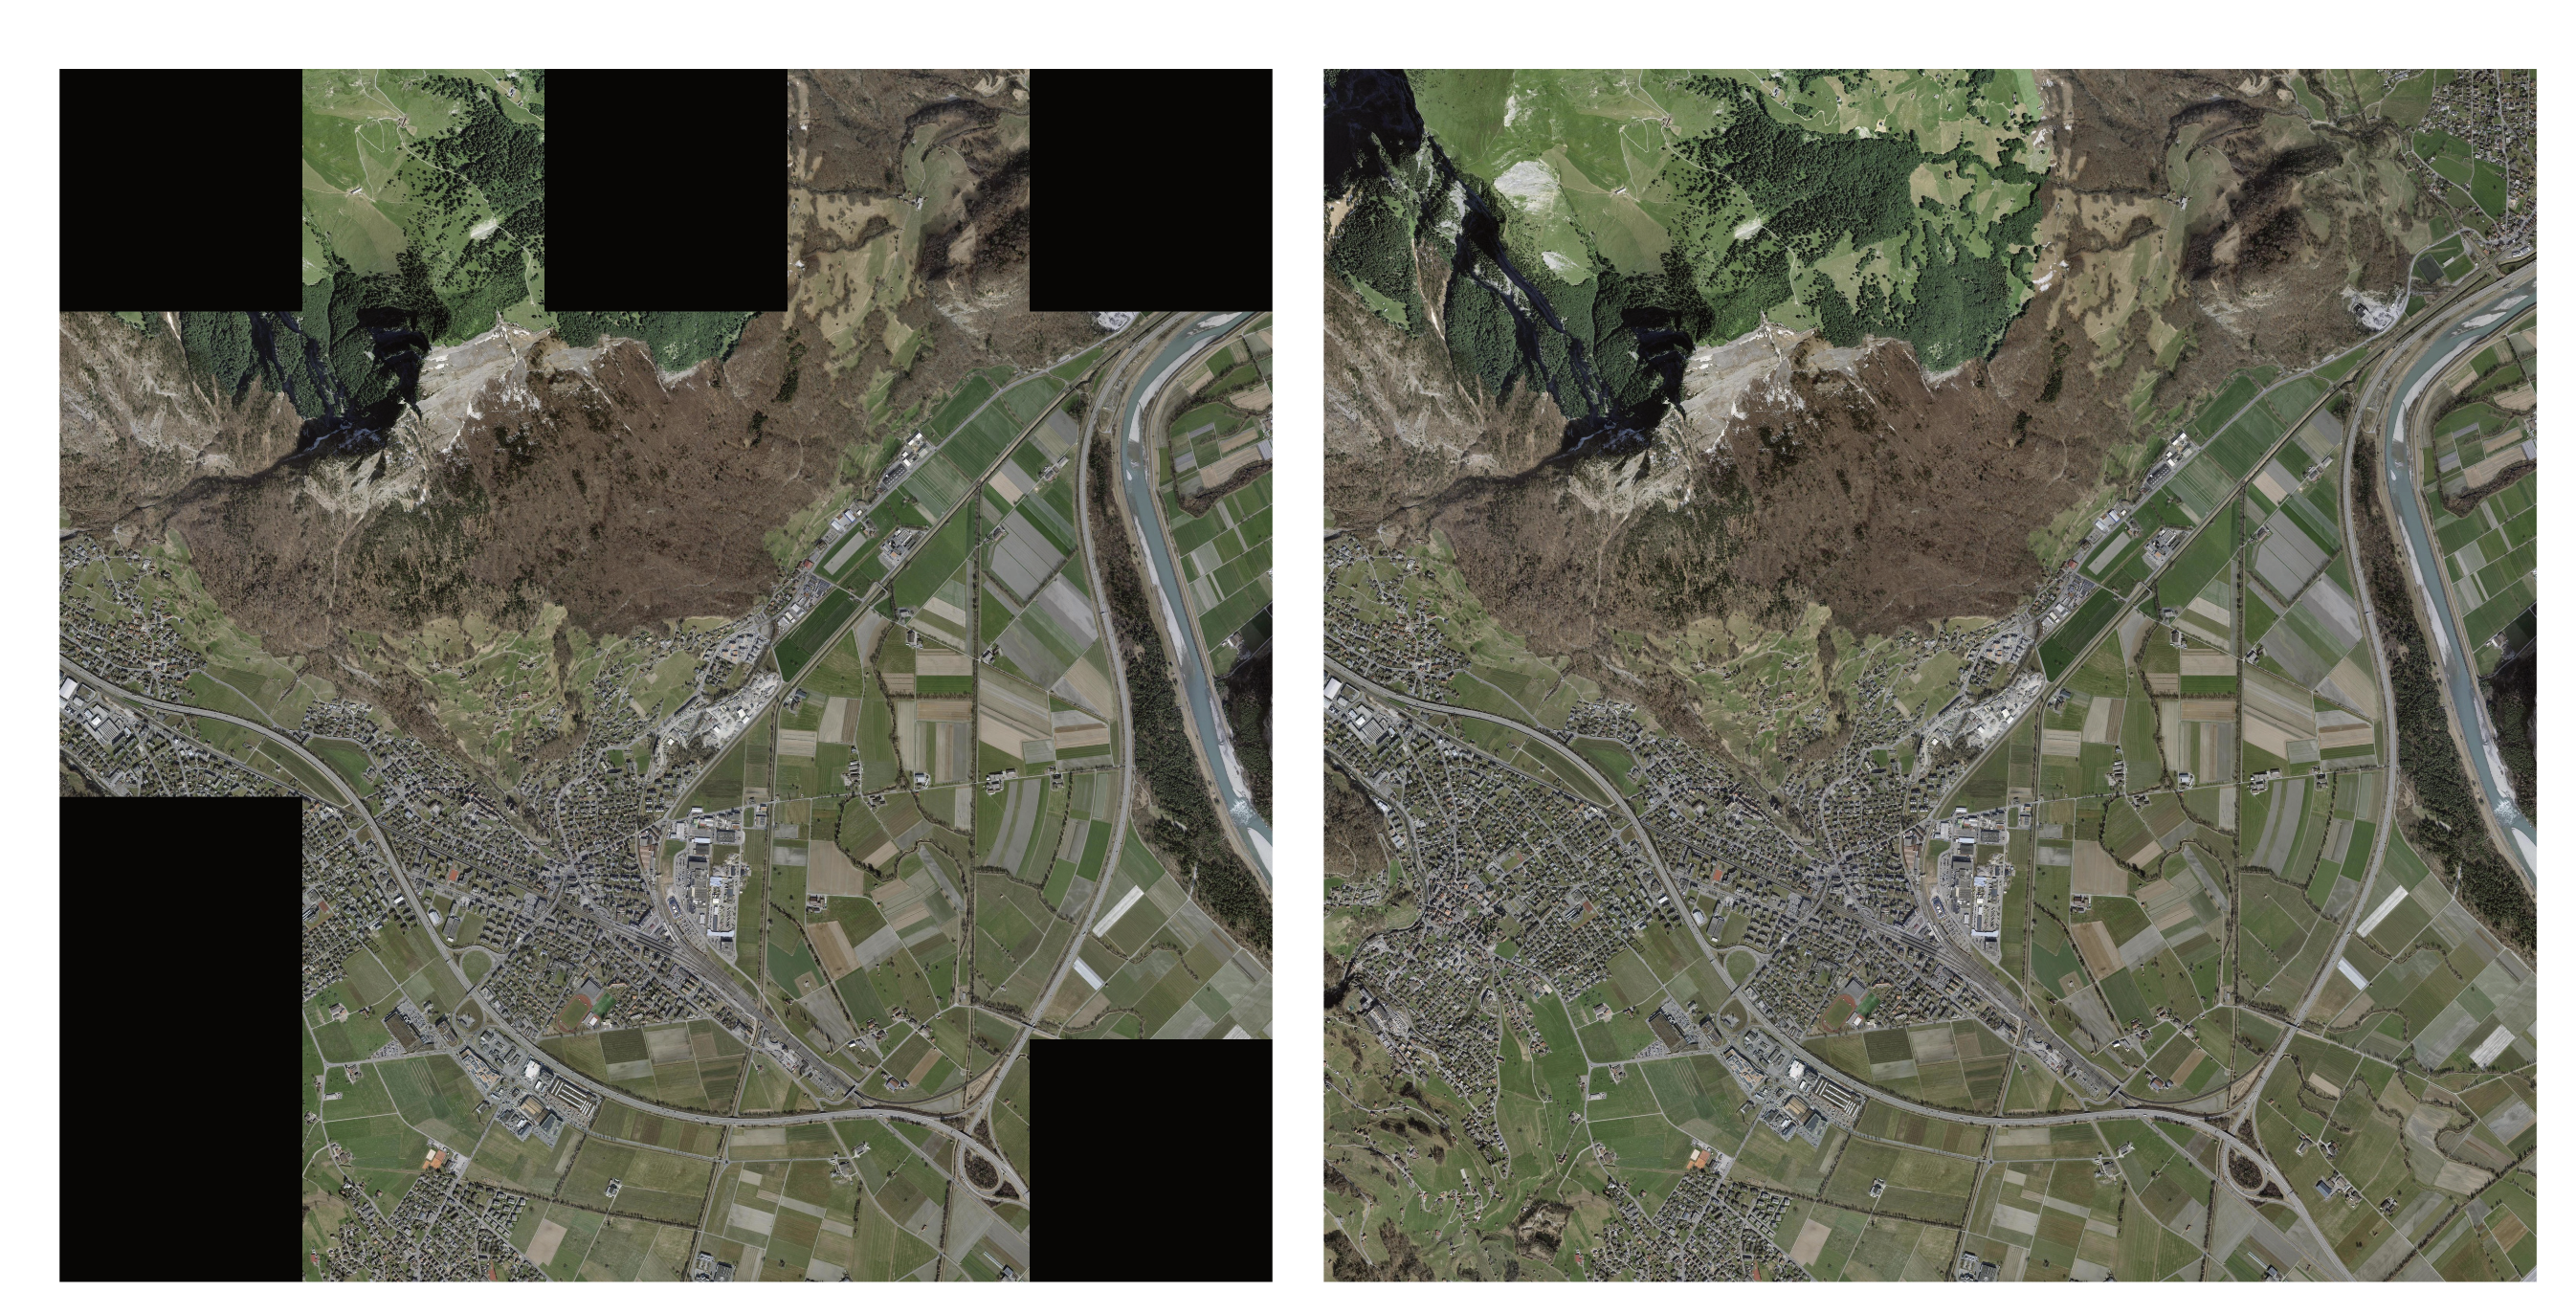
\includegraphics[width=.6\linewidth]{content/00_assets/gesamtbild_mit_luecken.png}
    \label{fig_swisstopo_daten_luecken}
\end{figure}

\subsection{Extrahierung der Höhen- und Bilddaten}
Sind die Daten heruntergeladen, müssen sowohl die Bild- als auch die Höhenwerte aus den GeoTIFF-Dateien extrahiert und als eigenständige Texturen (Bilder) abgespeichert werden. Die Höhenwerte werden hierbei als Graustufenbild gespeichert. Eine weisse Farbe bedeutet hierbei einen hohen, schwarz einen tieferen Wert (siehe Abbildung \ref{fig_heightmap_beispiel}). 
\begin{figure}[H]
    \caption{Extrahierte Höhenwerte als Graustufenbild (Eigene Darstellung)}
    \includegraphics[width=.4\linewidth]{content/00_assets/heightmap_beispiel.png}
    \label{fig_heightmap_beispiel}
\end{figure}

Um die Geopositionsdaten nicht zu verlieren, werden diese in den Dateinamen geschrieben. Da die Daten von swisstopo in Form von km$^2$-Kacheln zur Verfügung gestellt werden, müssen die Kacheln in einem nächsten Schritt zu einem Gesamtbild zusammengesetzt werden. Da die Geoposition jeder Kachel anhand des LV95-Koordinatensystems bekannt ist, können diese anhand der zugehörigen Nord- und Ostachsenwerte zusammengesetzt werden. Hier offenbart sich jedoch das erste Problem mit den Höhenwerten. Jede Kachel besitzt einen eigenen minimalen sowie maximalen Höhenwert. Werden die einzelnen Kacheln als Graustufenbilder zusammengesetzt, so gibt es keine fliessenden Übergänge. Um dieses Problem zu lösen, wurden die Höhenwerte anhand des globalen Minimums und Maximums normalisiert (siehe Abbildung \ref{fig_heightmap_sargans}).
\begin{figure}[H]
    \caption{Zusammengesetzten Graustufenbild von Sargans mit fliessenden (links) und nicht fliessenden Übergängen (Eigene Darstellung)}
    \includegraphics[width=.7\linewidth]{content/00_assets/heightmap_sargans.png}
    \label{fig_heightmap_sargans}
\end{figure}

Das Extrahieren der Farbwerte aus dem swissIMAGE Datensatz ist einfacher, da hierbei lediglich die Farbwerte aus den einzelnen Kacheln herausgelesen werden müssen und keine Normalisierung notwendig ist (siehe Abbildung \ref{fig_textur_sargans}). Aufgrund unterschiedlicher Aufnahmezeiträume können jedoch visuelle Diskrepanzen wie im Bereich A (siehe Abbildung \ref{fig_textur_sargans}) entstehen.
\begin{figure}[H]
    \caption{Zusammengesetztes von Sargans (Eigene Darstellung)}
    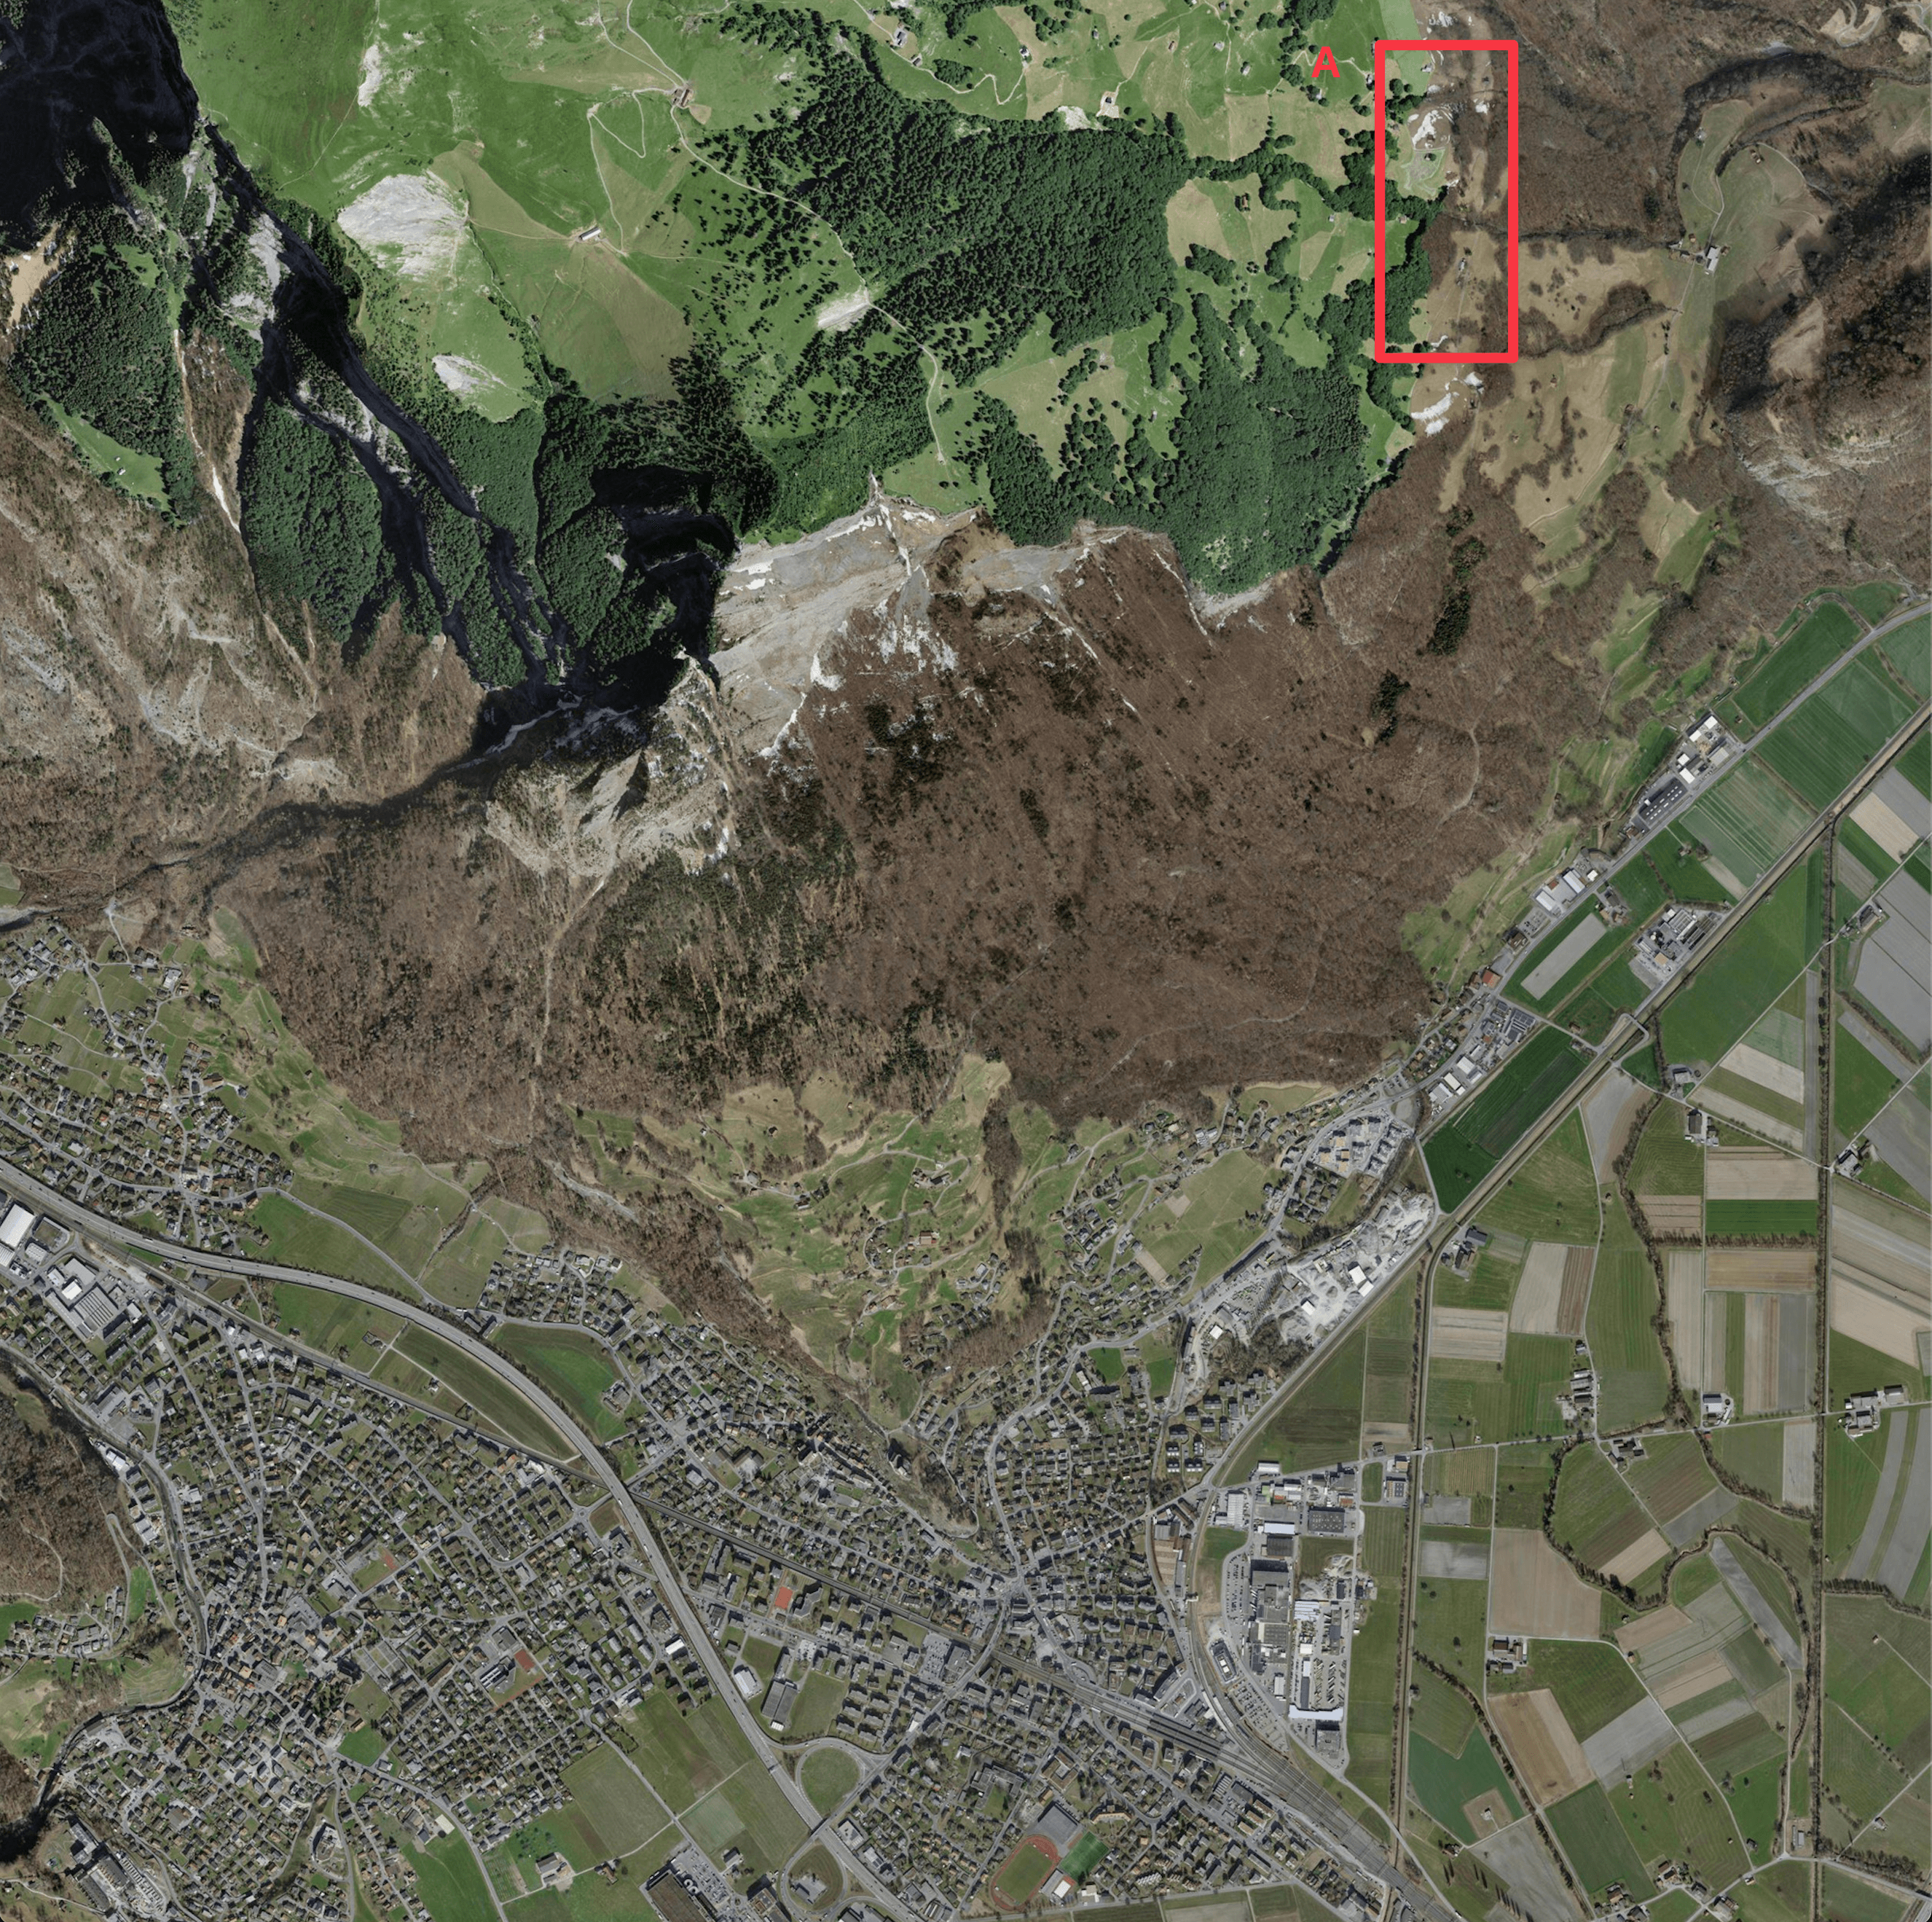
\includegraphics[width=.4\linewidth]{content/00_assets/textur_sargans.png}
    \label{fig_textur_sargans}
\end{figure}

\subsection{Aufteilung in kleinere Bilddateien}
Wie bereits in Kapitel \ref{chap_datengrundlage} angesprochen benötigen die Datensätze sowohl von swissALTI3D als auch swissIMAGE, abhängig von der gewählten Auflösung und Detaillierung, entsprechend viel Speicherplatz. Werden die einzelnen km$^2$ Kacheln für den Raum Sargans in der höchsten Auflösung von 10cm pro Bildpixel zu einem Gesamtbild zusammengesetzt, so werden rund 7.5GB Festplattenspeicher benötigt. Obwohl das für native Applikationen, sofern eine genügend schnelle Festplatte vorhanden ist, noch verkraftbar wäre, ist dies beispielsweise im Rahmen einer browserbasierten Anwendung nicht mehr tragbar. Browserbasierte Anwendungen haben gegenüber nativen Applikationen den Vorteil, dass sie von überall aus, ohne Installation, zugreifbar sind. Jedoch müssen die hierfür notwendigen Daten auch auf das Zielsystem des Nutzers heruntergeladen werden. Die Zeit hierfür hängt von der jeweiligen Internetbandbreite ab. Das Herunterladen von grossen Dateien ist daher meistens, trotz Konzepten wie Ladeanimationen etc., keine gute Idee. Um mit grossen Datenmengen auch im Rahmen von webbasierten Anwendungen umzugehen, gibt es andere Methoden.

Um das Problem mit den grossen Bildern zu lösen, wurden zwei Konzepte eingesetzt. Zum einen wurde das Gesamtbild in kleinere Bilddateien (auch Tiles genannt) unterteilt, zum anderen wurden diese mit einem bilinearen Downsampling auf eine maximale Auflösung limitiert. Die Tiles wurden hierbei, inspiriert von der Quadtree-Datenstruktur, erstellt. Genauso wie es bei einem Quadtree eine entsprechende Baumtiefe gibt, so gibt es bei den Teilbildern ebenfalls unterschiedliche Detaillierungsstufen. Für die erste Stufe (LOD 1) wurde das Gesamtbild in 4 (4$^1$) gleich grosse Teile geschnitten. Für die zweite Stufe sind es hingegen 16 Teilbilder (4$^2$) und so weiter. Abbildung \ref{fig_textur_teilbilder_quadtree} zeigt, wie ein Gesamtbild in Teilbilder mit unterschiedlichen Detailstufen (LODs) aufgeteilt wird. Hierbei sei angemerkt, dass aus Platzgründen nicht alle Teilbilder der Detailstufe LOD2 dargestellt wurden.
\begin{figure}[H]
    \caption{Aufteilung in Teilbilder, angelehnt an die Quadtree Datenstruktur (Eigene Darstellung)}
    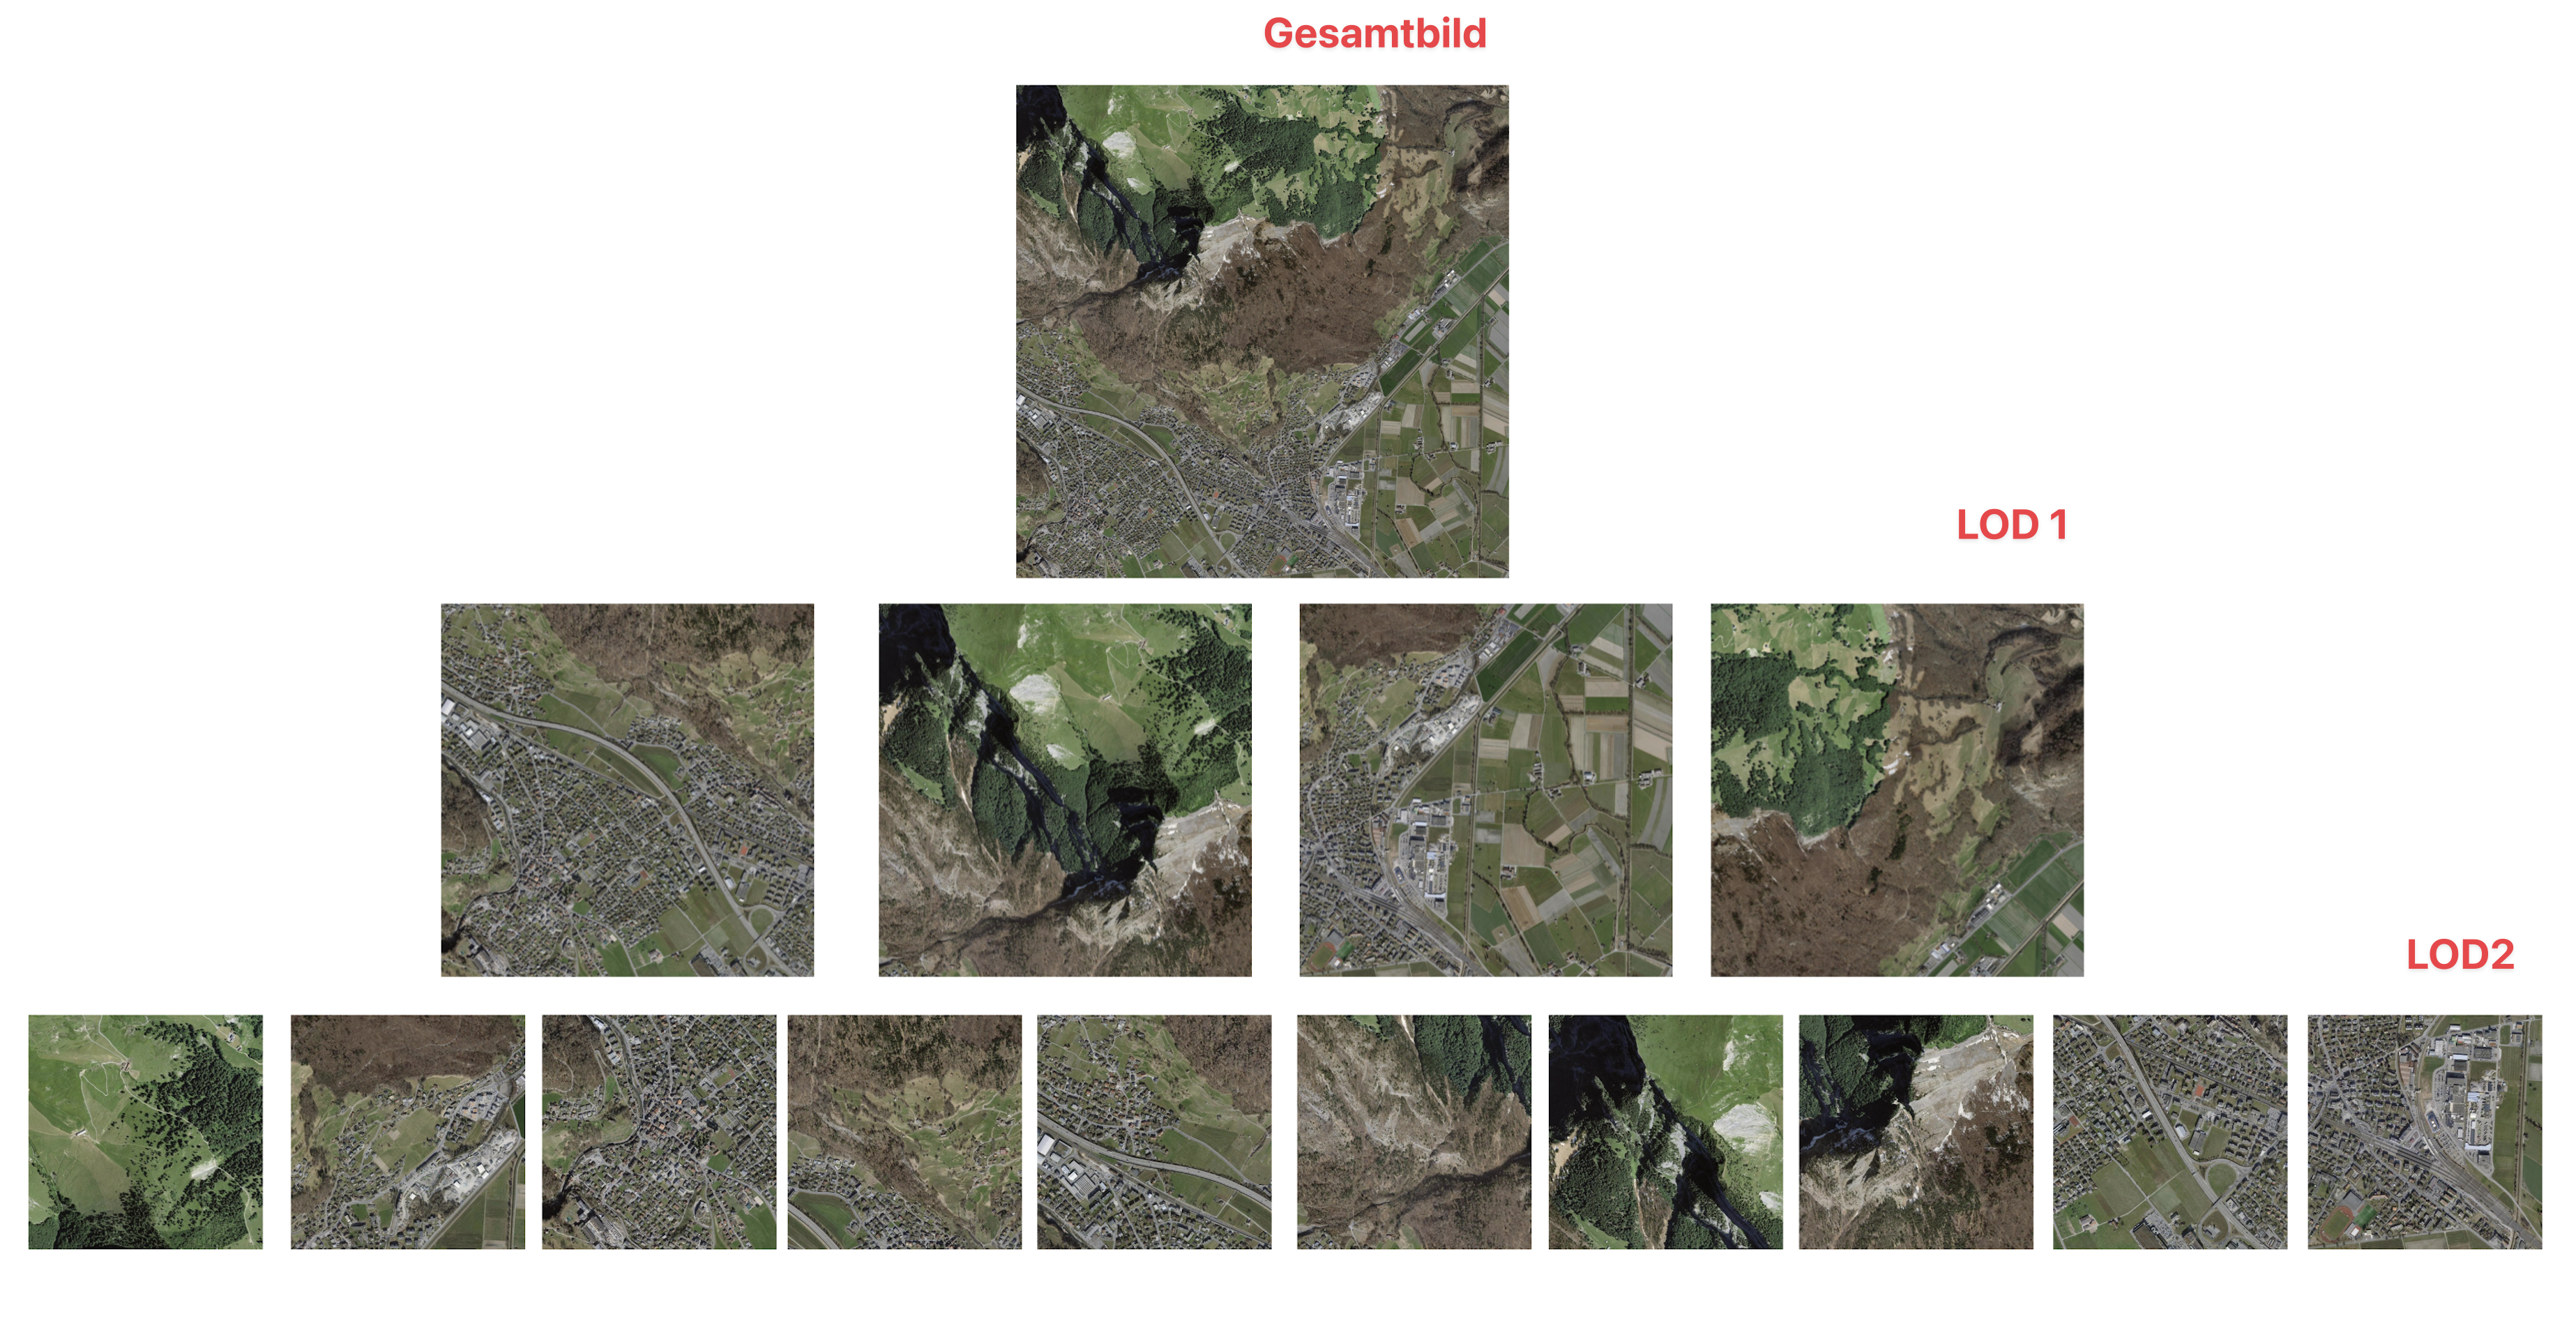
\includegraphics[width=1.0\linewidth]{content/00_assets/zerlegung_in_teilbilder.png}
    \label{fig_textur_teilbilder_quadtree}
\end{figure}

Grafikkarten bevorzugen aus Performanzgründen Texturen mit einer quadratischen Auflösung (500x500 etc.). Jedoch erstrecken sich die swisstopo-Daten je nach Region, nicht immer über einen quadratischen Bereich. Hierzu wird das zusammengesetzte Gesamtbild entsprechend auf einen quadratischen Bildausschnitt begrenzt (siehe Abbildung \ref{fig_begrenzung_bildausschnitt}). 
\begin{figure}[H]
    \caption{Begrenzung Bildausschnitt (Eigene Darstellung)}
    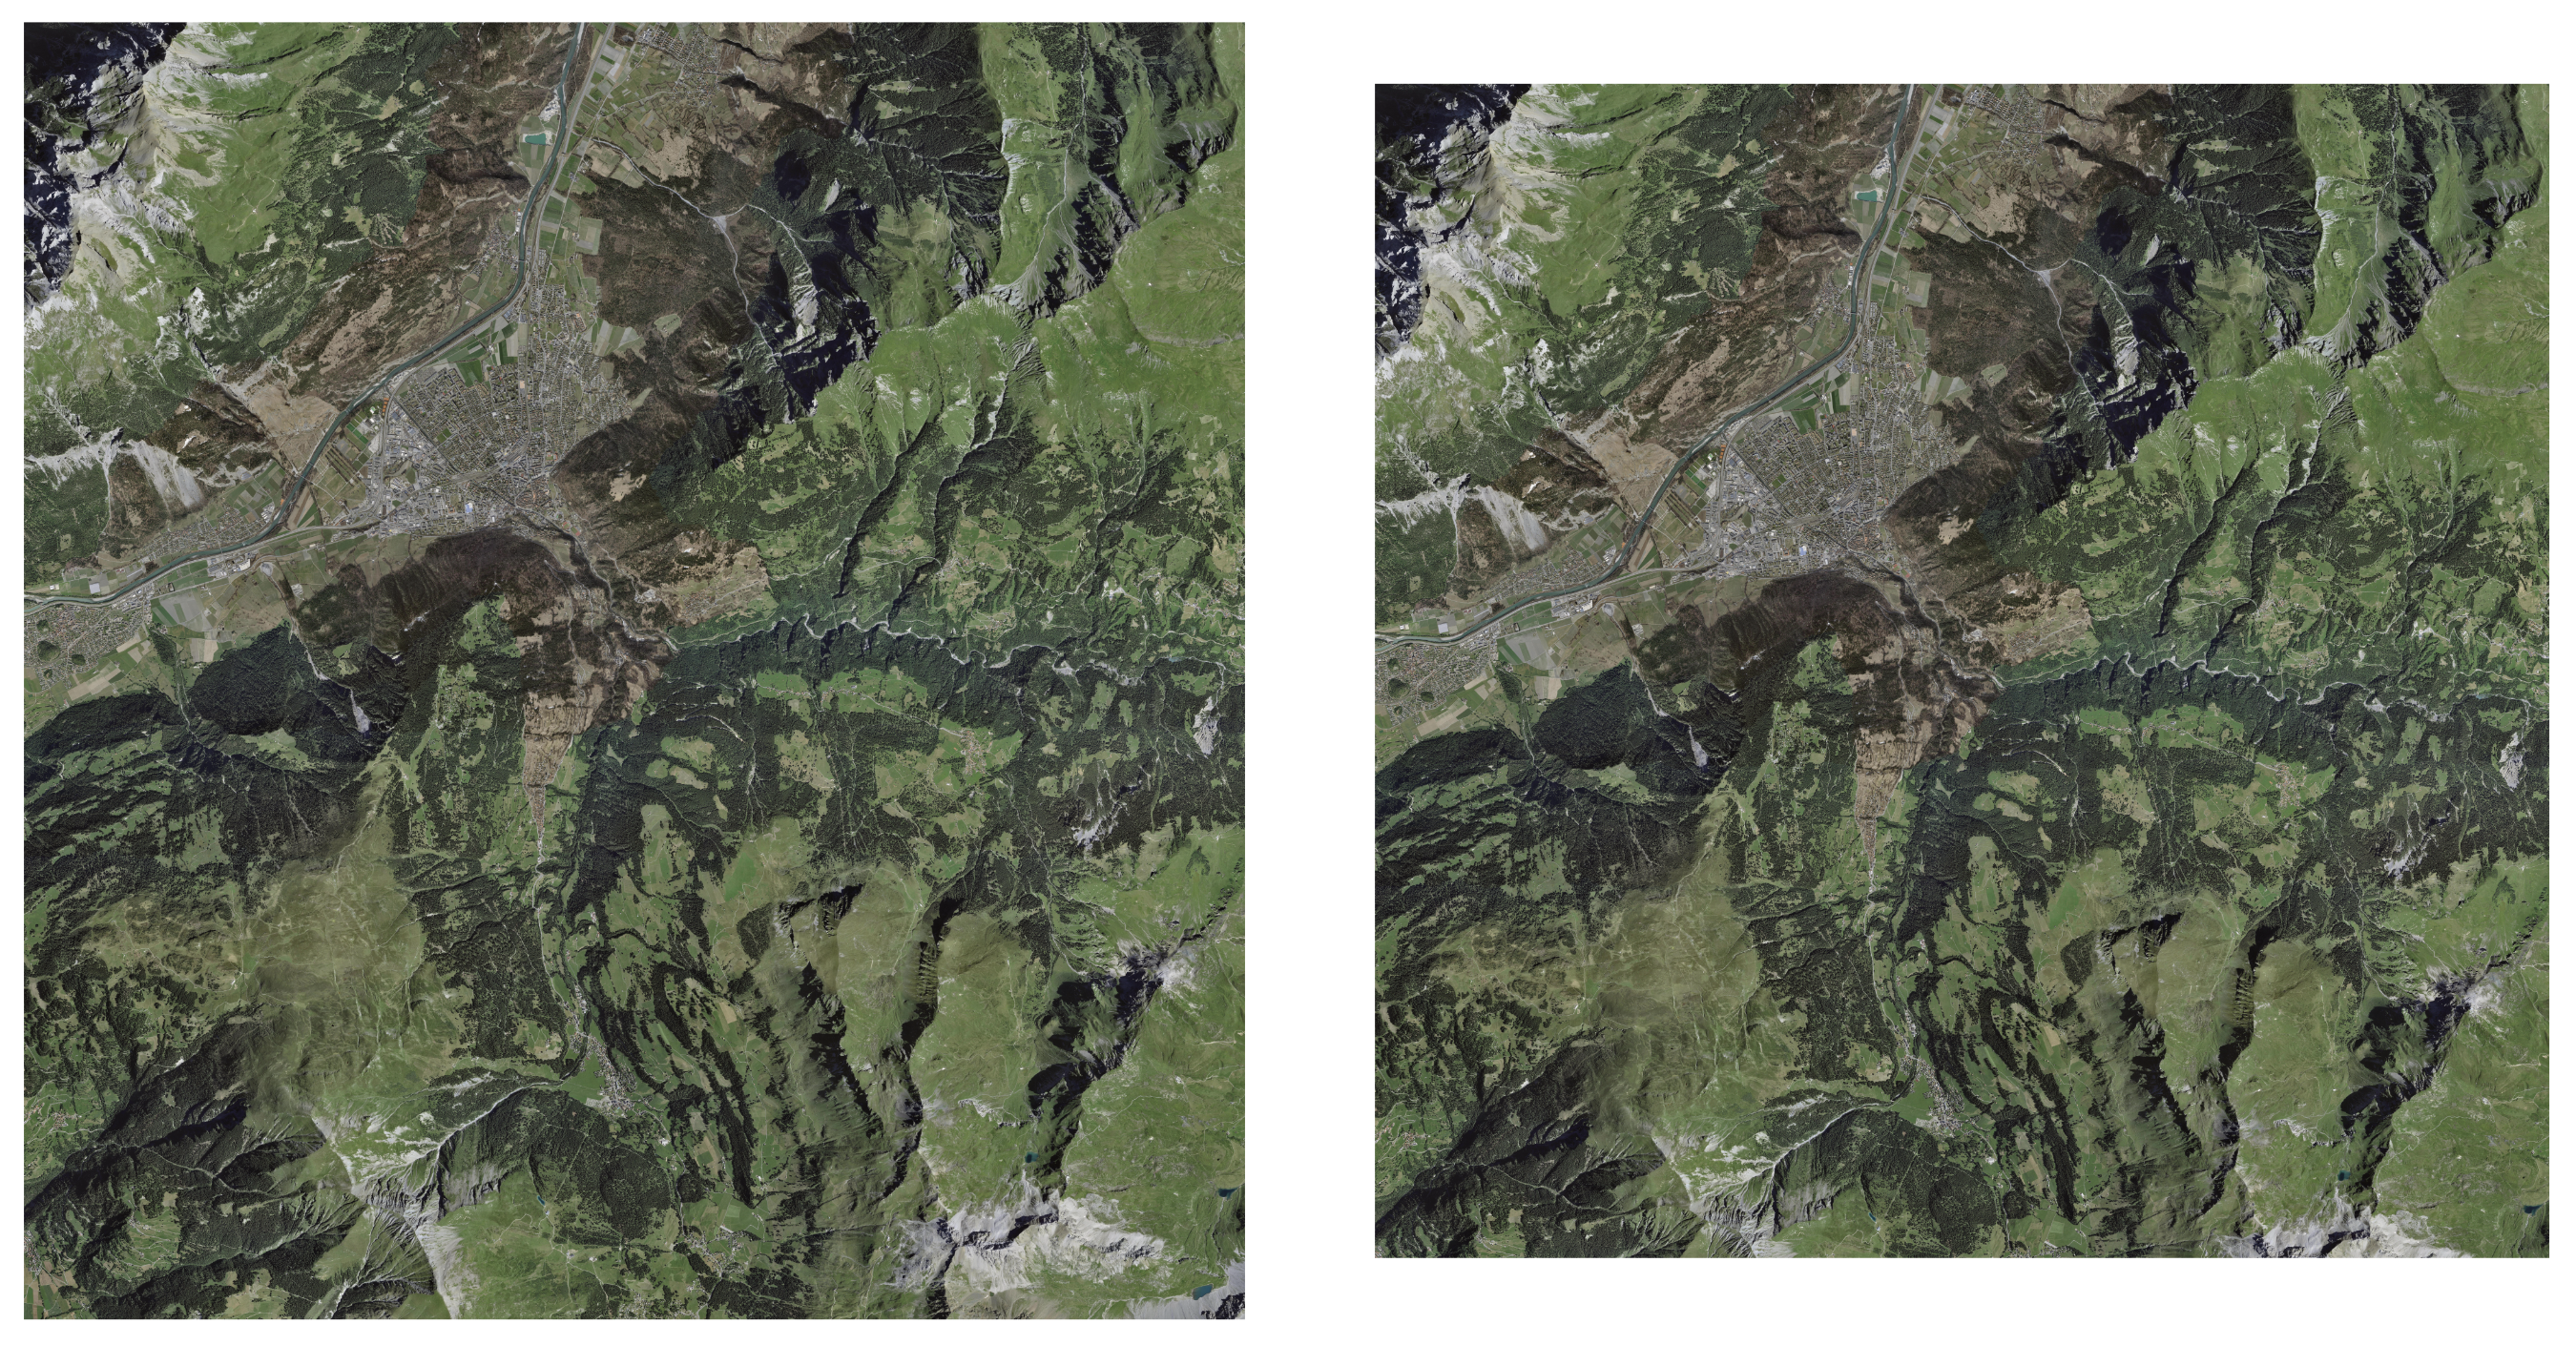
\includegraphics[width=.7\linewidth]{content/00_assets/begrenzung_bildausschnitt.png}
    \label{fig_begrenzung_bildausschnitt}
\end{figure}

\subsection{Automatische Ermittlung der maximalen Baumtiefe}
\label{chap_ermittlung_baumtiefe}
Die quadratische Begrenzung alleine reicht jedoch nicht aus. Da die Teilbilder anhand der Quadtree-Datenstruktur generiert werden, muss sichergestellt werden, dass in der höchsten Detailstufe (bspw. LOD2 in Abbildung \ref{fig_textur_teilbilder_quadtree}) das Gesamtbild restlos durch die Auflösung einer einzelnen km$^2$ Kachel teilbar ist. Hierfür wird die Logarithmusfunktion verwendet und anhand dieser automatisch die höchste Detailstufe ($L_{\max}$) und infolgedessen die Baumtiefe festgelegt. Hierzu ein Beispiel. Angenommen, das zusammengesetzte Luftbild von Sargans hat eine Auflösung ($R$) von 2000px auf 2000px. Wenn wir davon ausgehen, dass eine km$^2$ Kachel eine Auflösung von 2m pro Bildpunkt hat, ergibt sich somit eine Auflösung ($T$) von 500px ($\frac{1000m}{\frac{2m}{1px}}$) pro km$^2$. Mithilfe der unten stehenden Formel ergibt sich hiermit eine maximale Baumtiefe von 3.

\[
L_{\max} = (\log_2\frac{R}{T}) + 1
\]

\subsection{Border Patching}
Mithilfe der extrahierten Höhen sowie Bildinformationen ist es nun möglich, 3D-Modelle zu rekonstruieren. Auf die genaue Generierung der 3D-Modelle wird in Kapitel \ref{chap_erstellung_geometrie} eingegangen. Werden die 3D-Modelle aneinandergereiht, so wird jedoch ersichtlich, dass sich Risse an den angrenzenden Randbereichen bilden (siehe schwarze Bereiche in Abbildung \ref{fig_risse_zwischen_3d_modellen}). Grund hierfür ist folgender. Das Gesamtbild wird, wie bereits erwähnt, in Teilbilder zerschnitten. Die Höhendaten weisen jedoch an den entsprechenden Schnittkanten nicht die gleichen Werte wie ihre angrenzenden Nachbarn auf. Dementsprechend divergieren die Position der Vertices und es entstehen Risse.
\begin{figure}[H]
    \caption{Risse zwischen 3D Modellen der gleichen Detailstufe (Eigene Darstellung)}
    \includegraphics[width=.3\linewidth]{content/00_assets/risse_zwischen_gleichen_detailstufen.png}
    \label{fig_risse_zwischen_3d_modellen}
\end{figure}

Diese Problematik kann jedoch mithilfe von Broder Patching eliminiert werden. Die Idee hierbei ist, dass an den entsprechenden Rändern der Bilder jeweils Daten der angrenzenden Nachbarn übernommen werden und so ein Überlappungsbereich geschaffen wird. Ein Überlappungsbereich von bereits einem Pixel genügt, um die Risse komplett zu eliminieren. Der Überlappungsbereich ist in Abbildung \ref{fig_border_patching} rot hervorgehoben. An diesen Bereichen werden jeweils die Werte des angrenzenden Nachbarn (im Falle der Abbildung \ref{fig_border_patching} von 1 nach 2 etc.) übernommen.
\begin{figure}[H]
    \caption{Border Patching (Eigene Darstellung)}
    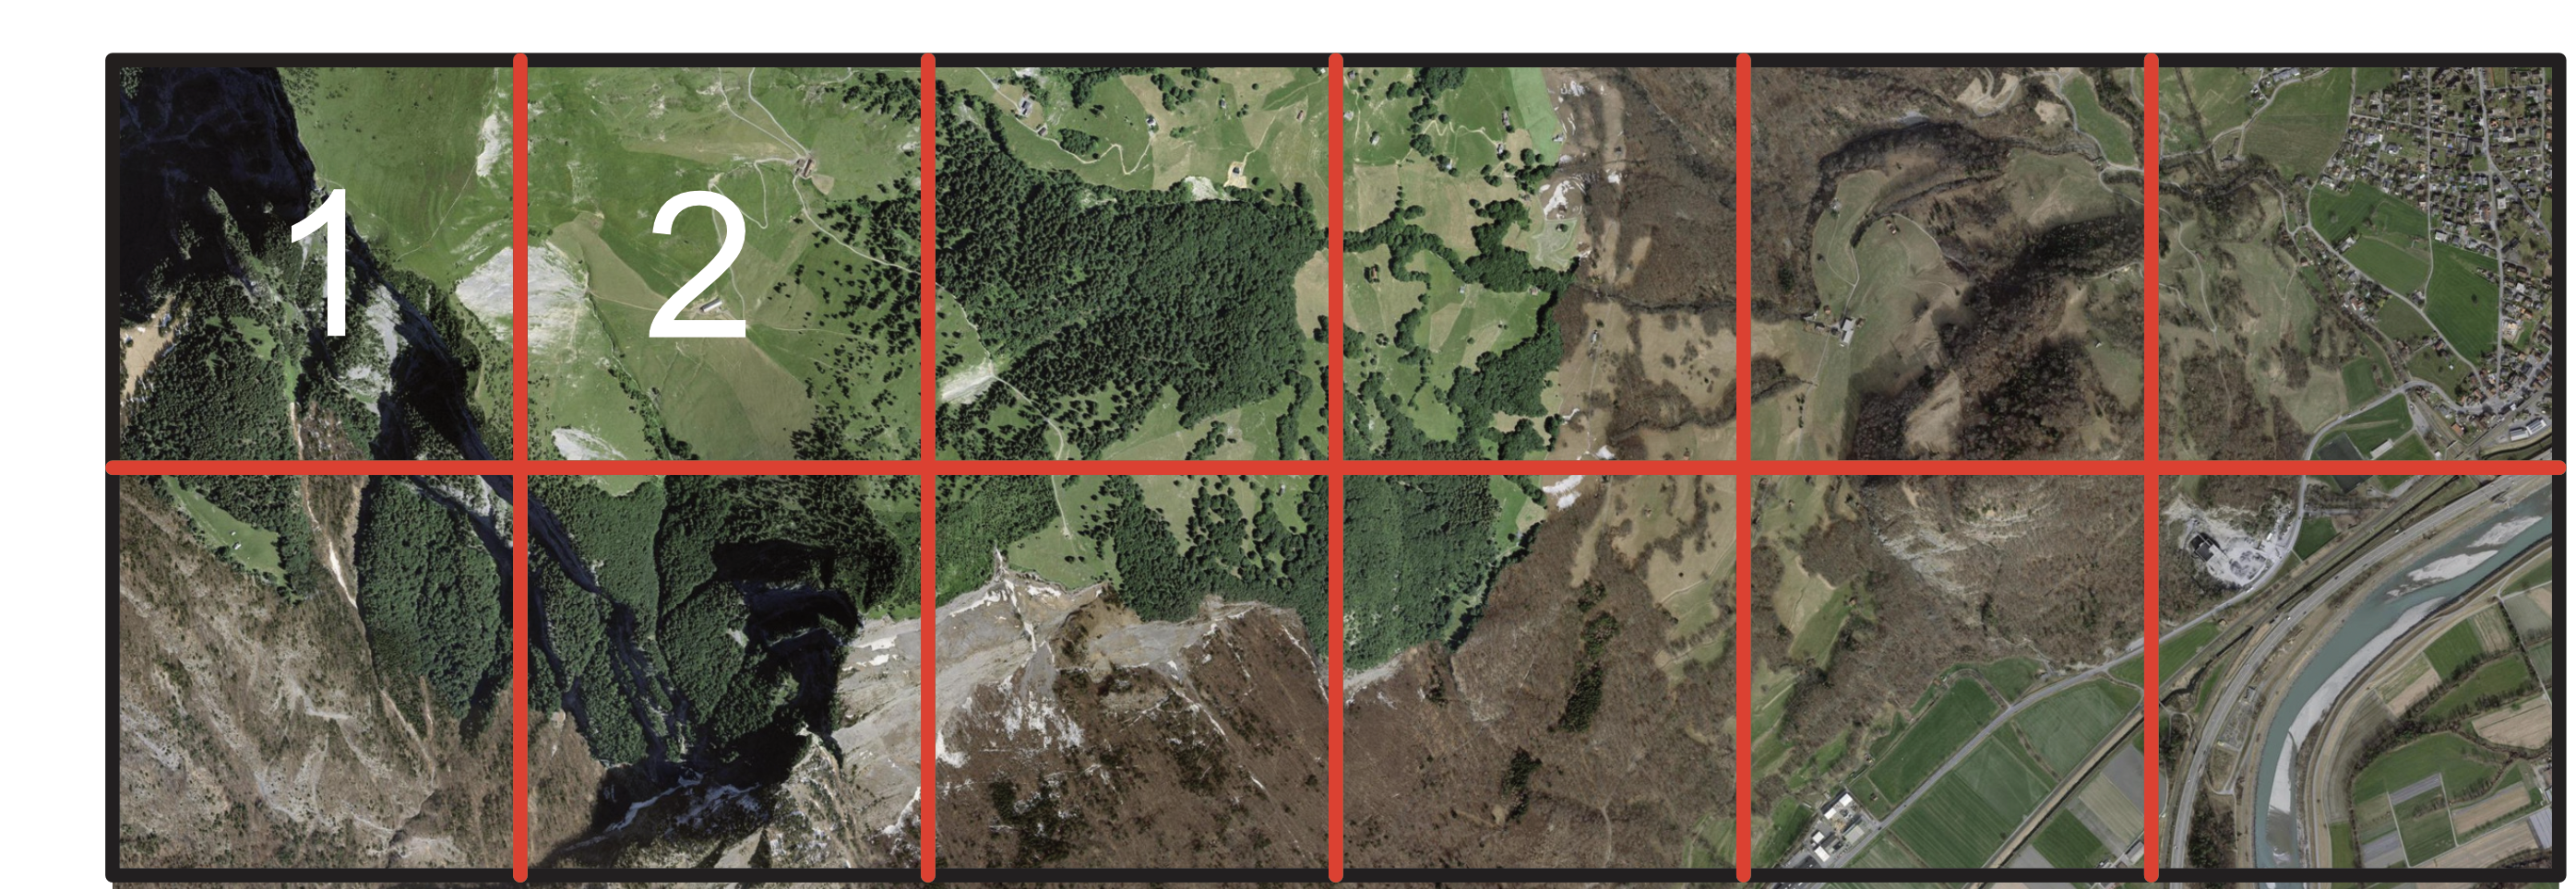
\includegraphics[width=.5\linewidth]{content/00_assets/border_patching.png}
    \label{fig_border_patching}
\end{figure}

\subsection{Relative Geopositionsinformationen}
ThreeJs hat wie die swisstopo-Daten einen Koordinatenursprung. Dieser Mittelpunkt befindet sich jedoch nicht wie bei swisstopo an den Koordinaten (2'600'000/1'200'000), sondern an der Stelle (0/0). Damit die 3D-Visualisierung um den ThreeJs Mittelpunkt positioniert werden kann, werden daher relative Geopositionsinformationen berechnet. Hierzu wird in einem ersten Schritt der Mittelpunkt des zusammengesetzten Gesamtbildes berechnet. Anschliessend wird bei der Erstellung der einzelnen Teilbilder der relative Abstand zu diesem Mittelpunkt bestimmt. Hiermit ist sichergestellt, dass die 3D-Modelle relativ um den ThreeJs Koordinatenursprung platziert werden können.

\subsection{Generierung von Metadaten}
\label{chap_generierung_metadaten}
Um wichtige Informationen zu den generierten Daten nicht zu verlieren, werden entsprechende Metadaten generiert. Diese werden in Form einer JSON-Datei abgespeichert und können somit zur Laufzeit der Webanwendung eingelesen werden. Abbildung \ref{fig_ausschnitt_metadaten} zeigt einen Ausschnitt aus den automatisch erstellten Metadaten. In den Metadaten stehen relevante Informationen wie:
\begin{itemize}
    \item Absolute Geopositionsinformationen im LV95-Koordinatensystem
    \item Relative Geopositionsinformationen im LV95-Koordinatensystem
    \item Maximale Baumtiefe (LOD)
    \item Globale Maximum und Minimum der Höheninformationen
    \item Dateipfade zu den generierten Bilddateien
\end{itemize}

\begin{figure}[H]
    \caption{Auszug aus den generierten Metadaten (Eigene Darstellung)}
    \includegraphics[width=.5\linewidth]{content/00_assets/ausschnitt_metadaten.png}
    \label{fig_ausschnitt_metadaten}
\end{figure}

\newpage

\section{Implementierung}
Dieses Kapitel widmet sich der eigentlichen Implementierung der 3D-Terrainvisualisierung auf Basis des ThreeJs Frameworks. Zu Beginn wird auf die Erstellung der eigentlichen 3D Modelle anhand der vorverarbeiteten swisstopo-Daten eingegangen. Anschliessend werden die eingesetzten Algorithmen sowie erstellte Hilfsvisualisierungen thematisiert. Abgerundet wird dieses Kapitel mit der Implementierung der Steuerungselemente zur freien Bewegung im 3D-Raum. 

\subsection{Erstellung der 3D-Geometrie}
\label{chap_erstellung_geometrie}
Um ein Gebirge in 3D darzustellen wird als geometrische Form ein Gitternetz von Punkten (Vertices) eingesetzt. Diese Gitternetze werden in ThreeJs als PlaneGeometry bezeichnet (siehe Abbildung \ref{fig_threejs_plane_geometry}). 
\begin{figure}[H]
    \caption{ThreeJs PlaneGeometry \parencite{threejs_beispiel_plane_geometry_2025}}
    \includegraphics[width=.3\linewidth]{content/00_assets/threejs_plane_geometry.png}
    \label{fig_threejs_plane_geometry}
\end{figure}

Jedoch spielt auch die Art und Weise, wie das Gitternetz erstellt wird, eine entscheidende Rolle. Um Risse im Terrain zwischen verschiedenen Detailstufen zu vermeiden, hat sich der Autor nicht für ein diagonales Muster wie in Abbildung \ref{fig_threejs_plane_geometry}, sondern für ein sternförmiges Muster (siehe Abbildung \ref{fig_plane_geometry_star_structure}) entschieden. Mithilfe dieser sternförmigen Struktur können auf einfache Art und Weise  geometrische Diskrepanzen wie Risse vermieden werden (die genaue Erläuterung folgt in Kapitel \ref{chap_algorithmen}). 
\begin{figure}[H]
    \caption{Gitternetz mit sternförmiger Struktur \parencite[S. 54]{frostbite_terrain_rendering_2007}}
    \includegraphics[width=.3\linewidth]{content/00_assets/geometry_star_pattern.png}
    \label{fig_plane_geometry_star_structure}
\end{figure}

Obwohl ThreeJs viele 3D-Geometrien bereits zur Verfügung stellt, ist es ebenso möglich, eigene 3D‑Geometrien zu erstellen. Hierzu stellt ThreeJs die Klasse \textit{BufferGeometry} zur Verfügung. Wie in Kapitel \ref{chap_render_pipelines} erwähnt, bestehen 3D-Modelle aus Dreiecken, welche wiederum aus Punkten (Vertices) bestehen. Um die Reihenfolge festzulegen, wie die einzelnen Punkte zu diesen Dreiecken zusammengesetzt werden, stehen sogenannte \textit{Indices} zur Verfügung. Hierzu ein Beispiel mit Bezug auf Abbildung \ref{fig_create_geometry_with_indices}. Um das Dreicke $abi$ zu erstellen, muss zuerst der Punkt $a$ mit dem Punkt $b$ und schlussendlich mit dem Punkt $i$ verbunden werden. Dies wird für sämtliche Dreiecke gemacht, bis die gewünschte sternförmige Struktur entsteht. 
\begin{figure}[H]
    \caption{Erstellung der Geometrie mittels Indices (Eigene Darstellung)}
    \includegraphics[width=.7\linewidth]{content/00_assets/erstellung_geometry_mittels_indices.png}
    \label{fig_create_geometry_with_indices}
\end{figure}

Momentan befinden sich jedoch die einzelnen Punkte alle noch auf einer Ebene. Um ein 3D-Modell zu erhalten, müssen die Punkte anhand der extrahierten swissALTI3D-Daten entsprechend nach oben oder unten verschoben werden. Die Verschiebung dieser Punkte erfolgt im Vertex Shader (siehe Kapitel \ref{chap_render_pipelines}). Hierbei werden die einzelnen Pixel aus dem Graustufenbild gelesen und anhand der vorberechneten globalen Maximum- und Minimumhöhe entsprechend skaliert. Anschliessend werden die Punkte anhand dieses Höhenwertes entsprechend nach unten oder oben verschoben (siehe Abbildung \ref{fig_verschiebung_punkte_vertex_shader}). Der Code in Abbildung \ref{fig_verschiebung_punkte_vertex_shader} ist hierbei in einer Three.js spezifischen Programmiersprache für Shader mit dem Namen \acrfull{TSL} geschrieben. Wie in Kapitel \ref{chap_technologien} thematisiert unterstützt Three.js sowohl WebGL als auch dessen Nachfolger WebGPU. Jedoch ist die Programmiersprache dieser zwei Technologien unterschiedlich. \acrshort{TSL} fungiert hier als Mediator zwischen diesen Sprachen und erlaubt es somit, beide Grafikschnittstellen anzusprechen. Dies hat den Vorteil, dass je nach Hardwaresupport entweder WebGL oder WebGPU von Three.js ausgewählt wird, der entsprechende Shader-Code aber nur einmal implementiert werden muss. 
\begin{figure}[H]
    \caption{Verschiebung der Punkte im Vertex Shader (Eigene Darstellung)}
    \includegraphics[width=.9\linewidth]{content/00_assets/positionierung_punkte_vertex_shader.png}
    \label{fig_verschiebung_punkte_vertex_shader}
\end{figure}

\subsection{Texturierung der 3D-Geometrie}
\label{chap_texturierung_3d_geometrie}
Um 3D-Elemente in Three.js darzustellen benötigt Three.js nebst der eigentlichen Geometrie auch eine zugehörige Textur. In Three.js werden Texturen als \textit{Materials} bezeichnet. Die Geometrie alleine gibt dem 3D-Modell nur die notwendige Struktur, die Textur, welche über die Geometrie gelegt wird, gibt dem 3D-Modell schlussendlich sein finales Erscheinungsbild. Eine \textit{Material} in Three.js muss nicht zwingend eine Bilddatei sein, sondern kann auch durch eine Farbe repräsentiert werden. Um beispielsweise in Three.js einen Würfel in grüner Farbe darzustellen, werden lediglich eine \textit{BoxGeometry} sowie ein \textit{MeshBasicMaterial} mit der entsprechenden Farbe benötigt (siehe Abbildung \ref{fig_threejs_box}).
\begin{figure}[H]
    \caption{Beispielcode zur Erstellung eines Würfels in Three.js \parencite{threejs_beispiel_box_geometry_2025}}
    \includegraphics[width=.9\linewidth]{content/00_assets/threejs_beispiel_box.png}
    \label{fig_threejs_box}
\end{figure}

Analog zum Beispiel mit dem Würfel kann auch ein Gebirge mit einer Textur versehen werden. Die Texturen sind in diesem Fall die orthografisch korrigierten Luftbilder aus dem swissIMAGE-Datensatz. Hierzu werden im Fragment Shader (siehe Kapitel \ref{chap_render_pipelines}) die entsprechenden Pixelwerte der Luftbilder ausgelesen und als Farbe dargestellt. Das Endergebnis ist ein rekonstruiertes 3D-Modell (siehe Abbildung \ref{fig_texturiertes_3d_modell}) auf Basis einer Kombination von swissALTI3D (Höhendatensatz) sowie swissIMAGE (Bilddatensatz). 
\begin{figure}[H]
    \caption{Ausschnitt rekonstruiertes 3D-Modell auf Basis der swisstopo-Daten (Eigene Darstellung)}
    \includegraphics[width=.5\linewidth]{content/00_assets/texturiertes_3d_modell.png}
    \label{fig_texturiertes_3d_modell}
\end{figure}

\subsection{Quadtree Algorithmus}
\label{chap_algorithmen}
Als Hauptalgorithmus hat sich der Autor für einen Quadtree entschieden. Hauptgrund hierfür war die einfachere Implementierung im Vergleich zum Geometry Clipmap Algorithmus in Anbetracht der zur Verfügung stehenden Zeit. Wie in Kapitel \ref{chap_algorithmen} angesprochen, benötigt ein Quadtree ein Kriterium, welches festlegt, wann neue Nodes generiert werden. Hierfür wurde die Distanz der Kameraposition zum Mittelpunkt einer Node ausgewählt (siehe Abbildung \ref{fig_quadtree_split_metric}). Zudem wurde der Quadtree anhand der vorberechneten Baumtiefe (siehe Kapitel \ref{chap_ermittlung_baumtiefe}) entsprechend limitiert. Der Quadtree erhält als Input die Länge sowie die Breite des Gebirges. Anschliessend wird periodisch (abhängig von der Bildwiederholrate) die Kameraposition in den Quadtree eingefügt und entsprechend die Abstände zu den einzelnen Nodes berechnet.
\begin{figure}[H]
    \caption{Quadtree Kriterium zur Erstellung neuer Nodes (Eigene Darstellung)}
    \includegraphics[width=.8\linewidth]{content/00_assets/quadtree_split_metric.png}
    \label{fig_quadtree_split_metric}
\end{figure}

\subsubsection{Assoziierung zu den Metadaten}
Die einzelnen Nodes der Quadtree Datenstruktur enthalten Informationen über das räumliche Gebiet sowie die dazugehörige Baumtiefe. Diese Informationen müssen mit den generierten Metadaten (siehe Kapitel \ref{chap_generierung_metadaten}) verknüpft werden, sodass die hinterlegten Texturen und schlussendlich die darauf basierenden 3D-Modelle erstellt werden können. Hierzu werden die Metadaten, welche als JSON-Datei abgespeichert wurden, initial beim Start der Webanwendung, geladen. Die Assoziierung einer Quadtree Node zu den Metadaten erfolgt anschliessend aufgrund des Zentrums der Quadtree Node sowie der Baumtiefe (siehe Abbildung \ref{fig_assoziierung_quadtree_node_metadaten}). 
\begin{figure}[H]
    \caption{Assoziierung Quadtree Node zu den Metadaten (Eigene Darstellung)}
    \includegraphics[width=.7\linewidth]{content/00_assets/assoziierung_quadtreenode_metadaten.png}
    \label{fig_assoziierung_quadtree_node_metadaten}
\end{figure}

Das Zentrum sowie die Baumtiefe werden aufgrund der erstellten Metadaten (siehe Kapitel \ref{chap_generierung_metadaten}) ermittelt. Das Zentrum wird anhand des Feldes \textit{bbox\_world\_space} berechnet, die Baumtiefe entspricht dem Feld \textit{level} (siehe Abbildung \ref{fig_ausschnitt_metadaten_tile}). Die eigentlichen 3D-Modellen zu den einzelnen Nodes des Quadtrees werden anschliessend aufgrund dieser assoziierten Metadaten wie in Kapitel \ref{chap_erstellung_geometrie} sowie \ref{chap_texturierung_3d_geometrie} beschrieben erstellt. Da sich die Struktur des Quadtrees abhängig von der Kameraposition ändert, wurde auch sichergestellt, dass die assoziierten 3D Modelle zu den Nodes entsprechend gelöscht werden.
\begin{figure}[H]
    \caption{Ausschnitt Tile Metadaten (Eigene Darstellung)}
    \includegraphics[width=.7\linewidth]{content/00_assets/ausschnitt_metadaten_tile.png}
    \label{fig_ausschnitt_metadaten_tile}
\end{figure}

\subsubsection{Visuelle Diskrepanz zwischen Nodes mit unterschiedlicher Baumtiefe}
\label{chap_visuelle_diskrepanz_zwischen_nodes}
Je nach Baumtiefe erstrecken sich die einzelnen Nodes über einen grösseren Bereich. Für jede Node wird hierbei die gleiche sternförmige Geometrie (siehe Kapitel \ref{chap_erstellung_geometrie}) verwendet.  Treffen Geometrien mit einer unterschiedlichen Baumtiefe aufeinander, entstehen visuelle Diskrepanzen in Form von Rissen (siehe rote Bereiche in Abbildung \ref{fig_visuelle_diskrepanzen_zwischen_unterschiedlichen_lod_leveln}). 
\begin{figure}[H]
    \caption{Visuelle Diskrepanzen zwischen Geometrien mit einer unterschiedlichen Baumtiefe \parencite{frostbite_terrain_rendering_2007}}
    \includegraphics[width=.4\linewidth]{content/00_assets/lod_tjunctions.png}
    \label{fig_visuelle_diskrepanzen_zwischen_unterschiedlichen_lod_leveln}
\end{figure}

Die Risse entstehen, weil kleinere Geometrien zusätzliche Punkte aufweisen, welche nicht auf die Punkte der grösseren Geometrien passen. Diese zusätzlichen Punkte werden mithilfe des Vertex-Shaders ebenfalls nach unten oder oben verschoben, wodurch sich Risse bilden (siehe Abbildung \ref{fig_risse_zwischen_3d_modellen_unterschiedlicher_baumtiefe}).
\begin{figure}[H]
    \caption{Risse zwischen 3D Modellen unterschiedlicher Baumtiefe (Eigene Darstellung)}
    \includegraphics[width=.5\linewidth]{content/00_assets/risse_zwischen_unterschiedlichen_baumtiefen.png}
    \label{fig_risse_zwischen_3d_modellen_unterschiedlicher_baumtiefe}
\end{figure}

\newpage
Die Frostbite Engine bietet jedoch mithilfe des sogenannten \textit{Index-Stitchings} eine elegante Methode, um dieses Problem zu lösen. Wie in Kapitel \ref{chap_erstellung_geometrie} erwähnt erlauben \textit{Indices} festzulegen in welcher Art und Weise die einzelnen Dreiecke aus den Punkten zusammengesetzt werden. Mithilfe dieser Indices können auch einzelne Punkte übersprungen werden. Auf diesem Ansatz basiert das Index-Stitching der Frostbite Engine. Hierzu werden im Vorfeld rund neun unterschiedliche Permutationen berechnet. Diese Permutationen basieren auf der gleichen Grundgeometrie, haben jedoch an den Randbereichen unterschiedliche Indices (siehe Abbildung \ref{fig_frostbite_index_stitching}). Mithilfe dieser neun Geometrien lassen sich die Risse zwischen verschiedenen Baumtiefen komplett vermeiden.
\begin{figure}[H]
    \caption{Frostbite Engine Index-Stitching \parencite[S. 55]{frostbite_terrain_rendering_2007}}
    \includegraphics[width=.5\linewidth]{content/00_assets/frostbite_index_stitching.png}
    \label{fig_frostbite_index_stitching}
\end{figure}

Eine Limitation des Index-Stitching ist jedoch, dass sichergestellt sein muss, dass sich die Baumtiefe der einander grenzenden Nodes nur um maximal eine Stufe unterscheiden darf \parencite[S. 53]{frostbite_terrain_rendering_2007}. Sprich, der Quadtree muss entsprechend ausbalanciert sein.

\subsubsection{Hilfsvisualisierung}
Um sowohl die Korrektheit des Quadtrees als auch der Index-Stitching Methode zu überprüfen, wurde eine entsprechende Hilfsvisualisierung implementiert. Die einzelnen Nodes des Quadtrees werden hierbei als weisse Quadrate dargestellt. Die Bereiche welche mithilfe der Index-Stitching Methode entsprechend korrigiert werden müssen, sind durch rote Linien gekennzeichnet (siehe Abbildung \ref{fig_hilfsvisualisierung_quadtree_index_stitching}).
\begin{figure}[H]
    \caption{Hilfsvisualisierung für Quadtree und Index-Stitching (Eigene Darstellung)}
    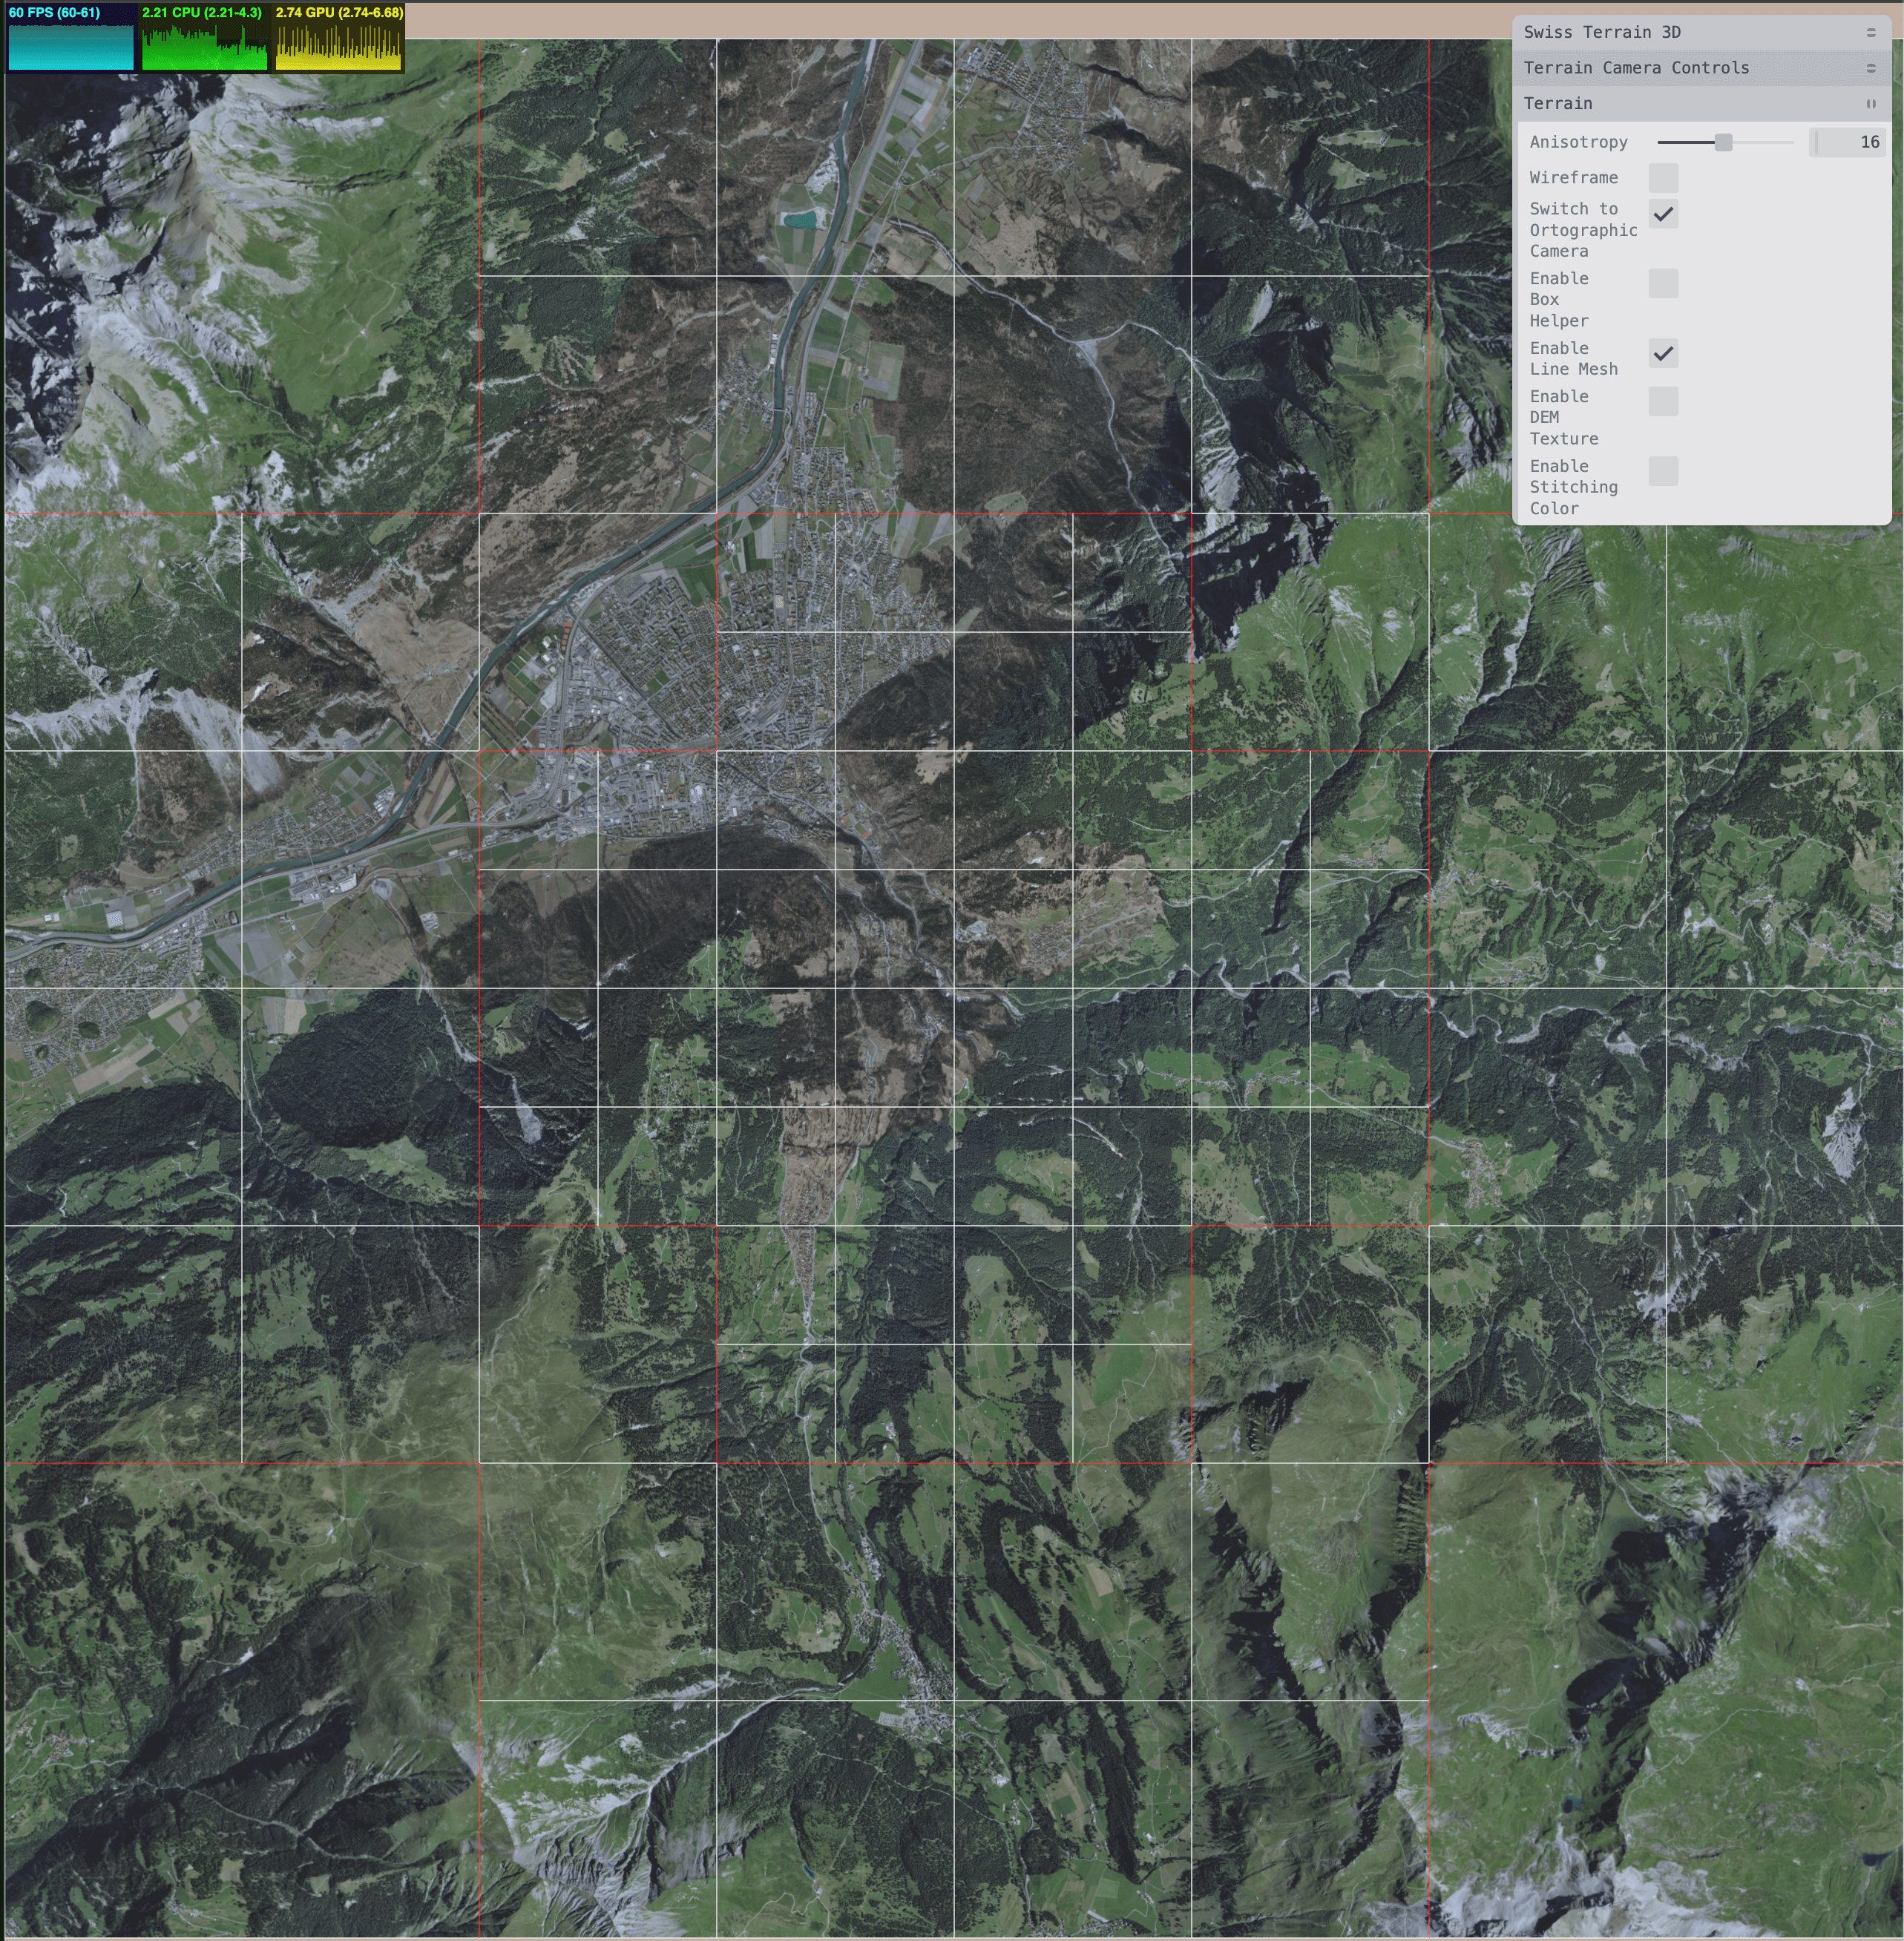
\includegraphics[width=.4\linewidth]{content/00_assets/hilfsvisualisierung_quadtree.png}
    \label{fig_hilfsvisualisierung_quadtree_index_stitching}
\end{figure}

Damit das Index-Stitching korrekt funktioniert, müssen für jede Node im Quadtree die angrenzenden Nachbarn sowie deren Baumtiefe ermittelt werden. Nachbarn mit derselben Baumtiefe können ignoriert werden. Je nachdem, auf welcher Kante die Nachbarn liegen, muss eine der Index-Stitching Permutationen ausgewählt werden (siehe Abbildung \ref{fig_auswahl_index_stitching}).
\begin{figure}[H]
    \caption{Ermittlung Index-Stitching (Eigene Darstellung)}
    \includegraphics[width=.5\linewidth]{content/00_assets/ermittlung_index_stitching_mode.png}
    \label{fig_auswahl_index_stitching}
\end{figure}

Abbildung \ref{fig_wireframe_index_stitching} zeigt eine Wireframe-Ansicht zweier angrenzender Geometrien mit einer unterschiedlichen Baumtiefe. Wie an den Rändern zu erkennen ist, gibt es bei der feingranularen Geometrie keine zusätzlichen Punkte mehr.
\begin{figure}[H]
    \caption{Wireframe Ansicht für Index-Stitching (Eigene Darstellung)}
    \includegraphics[width=.4\linewidth]{content/00_assets/index_stitching_wireframe.png}
    \label{fig_wireframe_index_stitching}
\end{figure}


\subsection{Steuerungselemente}
\label{chap_steuerungselemente}
Damit sich der Nutzer frei durch das Gebirge bewegen kann, müssen entsprechende Steuerungselemente implementiert werden. Der Betrachtungsausschnitt der Visualisierung wird hierbei durch eine Kamera definiert. In Three.js stehen verschiedene Arten von Kameras zur Verfügung. Eine perspektivische Kamera wird beispielsweise eingesetzt, um Objekte im 3D-Raum darzustellen. Hierbei erscheinen die entsprechenden Objekte abhängig von der Distanz entsprechend grösser oder kleiner. Die orthografische Kamera hingegen zeigt alle Objekte gleich gross dar (siehe Abbildung \ref{fig_threejs_cameras}). Eine perspektivische Kamera wird in der Visualisierung eingesetzt, um sowohl die Position als auch den Betrachtungsraum zu definieren. Die orthografische Kamera wird hingegen bei der Hilfsvisualisierung des Quadtree Algorithmus eingesetzt. 
\begin{figure}[H]
    \caption{Verschiedene Arten von Kameras in Three.js \parencite{threejs_exploring_cameras_2023}}
    \includegraphics[width=.5\linewidth]{content/00_assets/threejs_cameras.png}
    \label{fig_threejs_cameras}
\end{figure}

Mithilfe der Steuerungselemente werden sowohl die Position als auch der Betrachtungswinkel der Kameras  verändert und erlauben es so dem Nutzer, sich frei durch den 3D-Raum zu bewegen. Die Steuerung wurde hierbei mittels Tastatur und Maus umgesetzt. Die Tastatur erlaubt es, die Kameraposition zu verändern, wohingegen die Maus den Betrachtungswinkel beeinflusst. Tabelle \ref{table_steuerungselemente} zeigt eine Übersicht der Steuerungselemente und deren Auswirkung.
\begin{table}[H]
    \caption{Übersicht über Steuerungselemente und deren Auswirkung (Eigene Darstellung)}
    \begin{tabularx}{\textwidth} {
        >{\raggedright\arraybackslash}X 
        >{\raggedright\arraybackslash}X}
            \hline
            \textbf{Steuerungselement} & {Auswirkung}  \\
            \hline
            W-Taste oder Pfeiltaste nach oben & Bewegung nach vorne \\
            A-Taste oder Pfeiltaste nach link & Bewegung nach links \\
            S-Taste oder Pfeiltaste nach unten & Bewegung nach hinten \\
            D-Taste oder Pfeiltaste nach rechts & Bewegung nach rechts \\
            E-Taste & Bewegung nach oben \\
            R-Taste & Bewegung nach unten \\
            Mausbewegung & Veränderung des Betrachtungswinkels \\
            \hline
    \end{tabularx}
    \bigbreak
    \label{table_steuerungselemente}
\end{table}

\section{Ästhetik}
Three.js bietet diverse Möglichkeiten, um die Ästhetik einer 3D-Visualisierung zu beeinflussen. Ziel dieses Kapitels ist es, einen Überblick über die verwendeten ästhetischen Anpassungen zu geben sowie deren Einfluss zu erläutern.

\subsection{\acrfull{HDR} und Tone Mapping}
\acrfull{HDR} im Kontext von Bildern erlaubt es das Helligkeitsspektrum der einzelnen Farben, feingranularer darzustellen. Standardmässig sind die Farben eines Bildes nur innerhalb eines bestimmten Spektrums unterscheidbar. Farben, welche sich in den hellsten Bereichen des Spektrums befinden, werden weiss dargestellt, wohingegen Farben im niedrigsten Spektrum schwarz dargestellt werden. Die Spanne dieses Spektrums wird als Dynamic Range bezeichnet. Dadurch, dass diese Spannweite in \acrshort{HDR} erheblich grösser und feingranularer ist, werden die Helligkeitsunterschiede besser repräsentiert \parencite{hdr_2022}. Abbildung \ref{fig_terrain_hdr_no_hdr} zeigt die entsprechenden Unterschiede in der Darstellung der Helligkeitswerte.

\begin{figure}[H]
    \caption{Kontrastunterschied der Gebirge mit HDR (links) und ohne (rechts) (Eigene Darstellung)}
    \includegraphics[width=1.0\linewidth]{content/00_assets/terrain_hdr_no_hdr.png}
    \label{fig_terrain_hdr_no_hdr}
\end{figure}

Um \acrshort{HDR} Bilder zu erstellen, gibt es mehrere Möglichkeiten. Zum einen können die Bilder mithilfe des Computers erstellt werden. Jedoch ist es auch möglich, ein \acrshort{HDR} Bild auf Basis von mehreren normalen Bildern zu erstellen. Diese normalen Bilder sind in diesem Kontext auch unter dem Begriff \acrfull{SDR} bekannt. Ebenso ist es möglich, \acrshort{HDR} Bilder mithilfe von speziellen Kamerasensoren direkt zu erstellen \parencite{hdr_2022} oder über Webseiten wie Poly Haven\footnote{\url{https://polyhaven.com/hdris}} herunterzuladen.

Damit diese Werte jedoch auf einem Bildschirm dargestellt werden können, müssen sie zuerst in ein darstellbares Spektrum überführt werden. Um dies zu bewerkstelligen, wird Tone Mapping verwendet.
Three.js unterstützt hierbei verschiedene Tone Mapping-Verfahren. Abbildung \ref{fig_tone_mapping_threejs} zeigt hierbei die Auswirkungen von verschiedenen Tone Mapping Verfahren auf die finale Darstellung.

\begin{figure}[H]
    \caption{Verschiedene Tone Mapping-Verfahren in Three.js von links nach rechts (Kein Tone Mapping, Agx, Filmic, Reinhard) (Eigene Darstellung)}
    \includegraphics[width=.8\linewidth]{content/00_assets/tone_mapping_threejs.png}
    \label{fig_tone_mapping_threejs}
\end{figure}

\subsection{Anisotropy}
Um die Performance zu erhöhen, können für Texturen sogenannte Mipmaps erstellt werden. Mipmaps sind herunterskalierte Versionen der Originaltextur (siehe Abbildung \ref{fig_mipmaps}). Die Grafikkarte selektiert je nach Blickwinkel und Abstand die passende Mipmap Textur. Mit dieser Methode werden automatisch kleinere (herunterskalierte) Versionen für Dinge genutzt, welche sich in der Ferne befinden \parencite{mipmaps_2023}.
\begin{figure}[H]
    \caption{Mipmaps \parencite{mipmaps_2023}}
    \includegraphics[width=.3\linewidth]{content/00_assets/mipmaps.jpg}
    \label{fig_mipmaps}
\end{figure}

Jedoch kann es bei der Verwendung von Mipmaps dazu führen, dass Texturen, welche sich in der Ferne befinden, kaum mehr erkennbar oder unscharf erscheinen. Um dieses Problem zu lösen, gibt es die Möglichkeit, mithilfe der Anisotropy zu definieren, wie oft die einzelnen Bildpunkte einer Mipmap gefiltert werden sollen \parencite{threejs_anisotropy_2025}. Hiermit können verwaschene und unscharfe Texturen vermieden werden (siehe rote Bereiche A und B in Abbildung \ref{fig_anisotropy}).
\begin{figure}[H]
    \caption{Texturen mit Anisotropy (links) und ohne (rechts) (Eigene Darstellung)}
    \includegraphics[width=1.0\linewidth]{content/00_assets/textur_mit_anisotropy_ohne.png}
    \label{fig_anisotropy}
\end{figure}

\subsection{Procedural Sky}
Das Three.js Ökosystem bietet eine Vielzahl von verschiedenen Modulen an, um realitätsnahe Visualisierungen zu ermöglichen. Mithilfe des \textit{Procedural Sky}\footnote{\url{https://threejs.org/examples/?q=sky#webgpu_sky}} kann ein Tag- und Nachtzyklus simuliert werden. Das Procedural Sky Plugin von Three.js bietet hierbei diverse Einstellungsmöglichkeiten, womit wichtige Elemente wie die Sonnenposition etc. eingestellt werden können. Dies ermöglicht es, das 3D-Gebirge in einer realitätsnahen Umgebung in Szene zu setzen. Abbildung \ref{fig_procedural_sky} zeigt einen Ausschnitt des 3D Gebirges mit dem Procedural Sky Plugin. Das linke Bild stellt das Gebirge ohne Procedural Sky dar, das mittlere und rechte Bild zeigen das Gebirge mit Procedural Sky aber jeweils unterschiedlichen Sonnenpositionen.
\begin{figure}[H]
    \caption{3D Gebirge mit Procedural Sky Plugin (Eigene Darstellung)}
    \includegraphics[width=1.0\linewidth]{content/00_assets/threejs_procedural_sky.png}
    \label{fig_procedural_sky}
\end{figure}

\subsection{Einstellungsmöglichkeiten (Tweaks)}
Die bis anhin besprochenen ästhetischen Elemente besitzen eine Vielzahl von verschiedenen Parametern. Um ein Gefühl dafür zu bekommen, welche Auswirkungen die Parameter haben und wie sich dadurch die visuelle Repräsentation verändert, ist es wichtig, dass diese in Echtzeit mithilfe von entsprechenden GUI-Elementen verändert werden können. Um Einstellungsparameter mit entsprechenden GUI-Elementen zu verknüpfen, stehen diverse Bibliotheken zur Verfügung. Eine populäre Bibliothek in der Three.js-Community ist Tweakpane\footnote{\url{https://tweakpane.github.io/docs/}}. Tweakpane bietet eine Vielzahl von unterschiedlichen GUI-Elementen wie Range-Slider, Color-Picker oder Accordions an. Tweakpane stellt zudem eine einheitliche Darstellung dieser Elemente zwischen den einzelnen Browsern sicher und ermöglicht ebenfalls, diese Elemente mithilfe von Themes\footnote{\url{https://tweakpane.github.io/docs/theming/}} entsprechend anzupassen. Der primäre Vorteil von Tweakpane gegenüber den standardmässigen HTML5-GUI-Elementen besteht darin, dass auf einfache Art und Weise eine Verknüpfung von Einstellungsparametern mit den GUI-Elementen möglich ist. Um ein Dropdown für die Auswahl des Tone-Mappings zu erstellen, müssen lediglich die Auswahloptionen sowie die Aktion, welche ausgeführt werden soll, wenn ein Element selektiert wird, definiert werden (siehe Abbildung \ref{fig_tweaks_code}).
\begin{figure}[H]
    \caption{Definitionsstruktur für ein Dropdown in Tweakpane (Eigene Darstellung)}
    \includegraphics[width=.6\linewidth]{content/00_assets/tweaks_beispiel_code.png}
    \label{fig_tweaks_code}
\end{figure}

Durch diese einfache Handhabung können schnell neue Elemente für wichtige Parameter definiert werden. Abbildung \ref{fig_tweaks} zeigt diverse GUI-Elemente, mithilfe derer diverse Aspekte der Terrain-Visualisierung in Echtzeit angepasst werden können.
\begin{figure}[H]
    \caption{Tweaks der Terrain-Visualisierung (Eigene Darstellung)}
    \includegraphics[width=.3\linewidth]{content/00_assets/tweaks.png}
    \label{fig_tweaks}
\end{figure}

\section{Performanz}
Im Rahmen dieses Kapitels wird die Performanz der Visualisierung evaluiert. Ausgehend davon werden entsprechende Engpässe aufgedeckt und hierfür durchgeführte Optimierungen besprochen. Wichtig anzumerken ist, dass die Messung hierbei auf einem Macbook Pro M3 Max mit 64GB Arbeitsspeicher ausgeführt wurde und sich daher je nach Zielsystem entsprechend unterscheiden kann. 

\subsection{Im Vorfeld vorgenommene Optimierungen}
Bevor mit der Messung der effektiven Performanz begonnen wurde, sind bereits einige Optimierungen im Vorfeld vorgenommen worden.

\subsubsection{Webworker für Quadtree-Algorithmus}
Der Browser erlaubt standardmässig nicht das Ausführen von JavaScript-Code in mehreren Threads. Dies bedeutet, dass kostspielige Operationen die Visualisierung blockieren und so Verzögerungen auftreten können. Jedoch ist es mithilfe von \textit{Webworkern} möglich, kostspielige Operationen in einem anderen Thread auszuführen. Dies ist jedoch mit gewissen Limitationen verbunden. Der Code hat beispielsweise keinerlei Zugriff auf das \acrfull{DOM} des Browsers. Dies untersagt unter anderem das Laden von Texturen. Jedoch können browserunabhängige Algorithmen wie der Quadtree sehr wohl in Webworker ausgelagert werden. Hierdurch können sowohl die Berechnung des Quadtree als auch das notwendige Ausbalancieren im Hintergrund laufen, während der Main-Thread sich auf das Aktualisieren und Darstellen der Visualisierung fokussieren kann.

\subsubsection{Vorladen der Texturen}
Damit die Texturen der einzelnen Quadtree-Nodes nicht dynamisch nachgeladen werden müssen, werden diese bereits zum Start der Applikation geladen. Obwohl dies zu Beginn für eine längere Wartezeit sorgt, hat dies zur Laufzeit den Vorteil, dass die Bilder sofort verfügbar sind und es somit nicht zu Ladeverzögerungen kommt.

\subsubsection{Frustum Culling}
Wie in Kapitel \ref{chap_steuerungselemente} erwähnt, unterstützt Three.js verschiedene Arten von Kameras. Diese Kameras haben ein definiertes Sichtfeld (Frustum). Um Performanz zu sparen, werden Dinge, welche sich ausserhalb dieses Sichtfeldes befinden, nicht gezeichnet. Dies wird auch als Frustum Culling bezeichnet. Damit detektiert werden kann, ob sich ein Objekt innerhalb oder ausserhalb des Sichtfeldes befindet, nutzt Three.js sogenannte \textit{Bounding Spheres}. Da jedoch zur Laufzeit neue Geometrien erstellt werden, muss für diese neuen Geometrien die jeweilige Bounding Sphere entsprechend berechnet werden. Hierfür wird pro Geometrie jeweils eine \textit{Bounding Box} berechnet. Eine Bounding Box ist ein dreidimensionaler Bereich, welcher die 3D-Geometrie umschliesst (siehe rote Bereiche in Abbildung \ref{fig_bounding_boxes}).
\begin{figure}[H]
    \caption{Visualisierung der Bounding Box (Eigene Darstellung)}
    \includegraphics[width=.4\linewidth]{content/00_assets/terrain_bounding_boxes.png}
    \label{fig_bounding_boxes}
\end{figure}
Diese Bereiche werden aufgrund der globalen Minimum- und Maximumhöhe des Gebirges sowie der geometrischen Form berechnet. Auf Basis dieses Bereiches kann anschliessend die für das Frustum Culling notwendige Bounding Sphere berechnet werden (siehe Abbildung \ref{fig_berechnung_bounding_box}).

\begin{figure}[H]
    \caption{Berechnung der Bounding Box (Eigene Darstellung)}
    \includegraphics[width=.5\linewidth]{content/00_assets/berechnung_bbox.png}
    \label{fig_berechnung_bounding_box}
\end{figure}

\subsubsection{Vorberechnung der Geometrie}
Die Geometrie der einzelnen Quadtree Nodes ist für alle Nodes dieselbe. Die Geometrien unterscheiden sich nur in der Grösse sowie im Index Stitching Verfahren (siehe Kapitel \ref{chap_visuelle_diskrepanz_zwischen_nodes}). Dies bedeutet konkret, dass lediglich rund neun Geometrien, eine Geometrie pro Index Stitching, berechnet werden müssen, um das gesamte Gebirge darzustellen. Diese neun Geometrien werden zum Start der Applikation berechnet, sodass diese zur Laufzeit anschliessend nur noch den einzelnen Nodes zugewiesen werden müssen. Somit muss die Geometrieberechnung nicht zur Laufzeit erfolgen, es müssen lediglich die Position sowie die Skalierung der Geometrie entsprechend gesetzt werden.

\subsection{Messung}
Die Messung orientiert sich an den in Kapitel \ref{technologie_anforderungen} erwähnten Anforderungen, d.h. die Visualisierung muss mit mindestens 60 Bildern pro Sekunde auf einer Auflösung von 2k (2048px auf 1080px) laufen. Um sowohl die Bildwiederholrate als auch diverse andere wichtige Faktoren wie CPU- und GPU-Auslastung zu überwachen, wurde die Bibliothek stats-gl\footnote{\url{https://github.com/RenaudRohlinger/stats-gl}} verwendet. stats-gl lässt sich auf einfache Art und Weise in das Three.js Framework integrieren. In einem ersten Schritt müssen die Metriken definiert werden (siehe \textit{trackFPS} und \textit{trackGPU} in Abbildung \ref{fig_statsgl}). Anschliessend muss stats-gl initialisiert und entsprechend pro Frame aktualisiert werden.

\begin{figure}[H]
    \caption{Integration von stats-gl in Three.js (Eigene Darstellung)}
    \includegraphics[width=.4\linewidth]{content/00_assets/statsgl.png}
    \label{fig_statsgl}
\end{figure}

Richtig konfiguriert erlaubt stats-gl nun das Überwachen der vordefinierten Metriken in Echtzeit. Hierzu bietet stats-gl entsprechende Widgets an, welche die Werte in Form von Grafen darstellen (siehe Abbildung \ref{fig_threejs_statsgl}). Hierbei hat sich gezeigt, dass die Visualisierung problemlos selbst bei einer Auflösung von 5k mit 60 Bildern pro Sekunde dargestellt werden kann. 
\begin{figure}[H]
    \caption{Grafwidgets von stats-gl (Eigene Darstellung)}
    \includegraphics[width=.4\linewidth]{content/00_assets/threejs_statsgl.png}
    \label{fig_threejs_statsgl}
\end{figure}

\subsection{Identifikation von Engpässen}
Während der Navigation durch ein grösseres Gebirge (Region Chur) wurde festgestellt, dass vor allem mit dem neuen WebGPU-Backend von Three.js kleine Unterbrechungen auftreten können. Die Unterbrechungen treten immer dann auf, wenn neue Geometrien erzeugt werden müssen, sprich, wenn sich die Struktur des Quadtrees verändert. Mithilfe der integrierten Browser-Monitoring-Tools konnte hierbei festgestellt werden, dass rund 60\% der Zeit hierfür für die Methode \textit{build} verwendet wird (siehe Abbildung \ref{fig_webgpu_build_issue}). 
\begin{figure}[H]
    \caption{WebGPU Engpass in \textit{build} Methode (Eigene Darstellung)}
    \includegraphics[width=.5\linewidth]{content/00_assets/performance_issue_build_method.png}
    \label{fig_webgpu_build_issue}
\end{figure}

Diese Methode übersetzt den \acrshort{TSL} spezifischen Code (siehe Kapitel \ref{chap_erstellung_geometrie}) in die effektive Shadersprache (GLSL/WGSL). Die Übersetzung wird auf der CPU ausgeführt und kann bei langen Ausführungszeiten zu Performanzeinbussen führen. Auf dem WebGL-Backend ist eine solche Übersetzung nicht notwendig, da der Code direkt in der entsprechenden Sprache (GLSL) geschrieben wird. Ein weiterer Engpass, welcher sowohl im WebGPU- als auch im WebGL-Backend auftritt, ist das Dekodieren der Bilddateien. Abbildung \ref{fig_performance_issue_image_decode} zeigt, dass im WebGL-Backend hierfür rund 40\% der Ausführungszeit verwendet wird. 
\begin{figure}[H]
    \caption{Dekodieren der Bilddateien (Eigene Darstellung)}
    \includegraphics[width=.8\linewidth]{content/00_assets/performance_issue_image_decode.png}
    \label{fig_performance_issue_image_decode}
\end{figure}

\subsection{Optimierungen}
Um die Problematik mit der Übersetzung von TSL spezifischem Code auf die effektive Shadersprache zu lösen, wurde entschieden, das WebGL- anstelle des WebGPU-Backends zu verwenden. Zum aktuellen Zeitpunkt ist zwar das WebGPU-Backend die modernere Alternative, jedoch befindet es sich im Three.js-Ökosystem noch in der Entwicklungsphase und hat daher nicht die gewünschte Stabilität von WebGL. Three.js erleichtert hierbei die Umstellung des Backends. Grosse Teile des Codes mussten nicht modifiziert werden, lediglich Shader spezifischer Code musste aufgrund der Umstellung von TSL auf GLSL neu geschrieben werden. Abbildung \ref{fig_vertex_shader_glsl_tsl} zeigt hierbei die Unterschiede zwischen dem GLSL und TSL Code. Die Hauptfunktion des Codes ist die Transformation der 3D-Punkte anhand des Höhenbildes (siehe Kapitel \ref{chap_erstellung_geometrie}).
\begin{figure}[H]
    \caption{Unterschiede zwischen GLSL und TSL Code (Eigene Darstellung)}
    \includegraphics[width=.6\linewidth]{content/00_assets/terrain_vertex_shader_glsl_tsl.png}
    \label{fig_vertex_shader_glsl_tsl}
\end{figure}

Damit die Bilder für die Nutzung auf der Grafikkarte nicht dekodiert werden müssen, stehen spezielle Bildformate zur Verfügung. Eines dieser Bildformate ist das \acrfull{KTX} Format\footnote{\url{https://github.khronos.org/KTX-Specification/ktxspec.v2.html}}. Mithilfe dieses Formats werden die Bilder so vorbereitet, dass diese bereits in einem für die Grafikkarte optimalen Format vorliegen und nicht dekodiert werden müssen. Hierfür wurde die Datenvorverarbeitung entsprechend angepasst, sodass die Bilder im \acrshort{KTX}-Format erstellt werden.

\subsubsection{Zukünftige Optimierungsmöglichkeiten}
Mithilfe weiterer Tools wie SpectorJS\footnote{\url{https://spector.babylonjs.com/}} kann jedes einzelne Bild auf der Grafikkarte im Detail analysiert werden. Hierbei zeigt sich, dass pro Geometrie (Quadtree Node) jeweils ein Draw Call Befehl an die Grafikkarte gesendet wird. Abbildung \ref{fig_spectorjs_draw_calls} zeigt, dass beispielsweise für das Gebirge im Raum Chur rund 89 Draw Calls notwendig sind. Diese Zahl steigt mit der Anzahl der Quadtree Nodes und somit mit der Grösse des Gebirges. Bei grossen Gebirgen kann es somit vorallem auf leistungsschwachen Endgeräten wie Smartphones zu Engpässen kommen.
\begin{figure}[H]
    \caption{SpectorJS Anzahl Draw Calls für Raum Chur (Eigene Darstellung)}
    \includegraphics[width=.3\linewidth]{content/00_assets/spectorjs_draw_calls.png}
    \label{fig_spectorjs_draw_calls}
\end{figure}
Three.js bietet mithilfe des sogenannten \textit{Instance Renderings} eine elegante Lösung für dieses Problem. Das Konzept von Instance Rendering besteht darin, dass die gleiche Geometrie beliebig oft von der Grafikkarte gezeichnet werden kann. Diese Geometrien werden alle gleichzeitig innerhalb desselben Draw Calls gezeichnet (siehe Abbildung \ref{fig_threejs_instance_rendering}). Da es für die Terrain Visualisierung rund neun unterschiedliche Arten von Geometrien gibt, kann so die Anzahl der Draw Calls erheblich reduziert werden. Aus Zeitgründen wurde diese Optimierung jedoch nicht vorgenommen und kann im Rahmen einer zukünftigen Erweiterung umgesetzt werden.
\begin{figure}[H]
    \caption{Three.js Instance Rendering \parencite{threejs_instance_rendering_2025}}
    \includegraphics[width=.4\linewidth]{content/00_assets/threejs_instance_rendering.png}
    \label{fig_threejs_instance_rendering}
\end{figure}
